\documentclass[a4paper,12pt]{article}
\usepackage[T1,T2A]{fontenc}
\usepackage[utf8]{inputenc}
\usepackage[english,russian]{babel}
\usepackage{amsmath}
\usepackage{amsfonts}
\usepackage{amssymb}
\usepackage{tabularx}
\usepackage{graphicx}
\usepackage{epstopdf}
\usepackage{pstool} 
\usepackage[small]{caption}
\usepackage{lmodern}

\usepackage{xcolor}
\usepackage{hyperref}

\renewcommand{\rmdefault}{cmr} % Шрифт с засечками
\renewcommand{\sfdefault}{cmss} % Шрифт без засечек
\renewcommand{\ttdefault}{cmtt} % Моноширинный шрифт

\renewcommand{\theequation}{
	\arabic{section}.\arabic{equation}
}

\oddsidemargin	-1.5cm 
\topmargin		-2.7cm 
\textwidth		19.0cm 
\textheight		26.7cm

\newcommand{\D}{\displaystyle}

\righthyphenmin=2

\begin{document}
	
	\graphicspath{{figures/}}
	
	\baselineskip = 20 true pt \vspace{40mm} \large
	\begin{titlepage}
		\begin{center}
			Федеральное государственное бюджетное\\ образовательное
			учреждение высшего образования\\[0.5cm]
			Омский государственный университет им. Ф.М. Достоевского\\[3cm]
			
			Математическое моделирование\\ уравнений математической физики\\[2cm]
			Задание № 4\\[1cm]
			Численные методы решения краевой задачи для двумерного волнового уравнения\\[3cm]
Вариант №\ 2 - 13\\[2cm]
\end{center}

\begin{flushright}
Выполнил:\\
студент группы ФПБ-803\\
Хитринцева Валерия Вадимовна\\[3cm]
\end{flushright}

\begin{center}
Омск-2021
\end{center}
\end{titlepage}

%>>>>>>>>>>>>>>>>>>>>>>>>>>>>>>>>>>>>>>>>>>>>>>>>>>>>>>>>>>>>>>>>>>>>>>>>>>>>>>>>>>>>>>>>>>>>>>>>>>>>>>>
\setcounter{page}{2} 
\tableofcontents
\newpage
%>>>>>>>>>>>>>>>>>>>>>>>>>>>>>>>>>>>>>>>>>>>>>>>>>>>>>>>>>>>>>>>>>>>>>>>>>>>>>>>>>>>>>>>>>>>>>>>>>>>>>>>

%>>>>>>>>>>>>>>>>>>>>>>>>>>>>>>>>>>>>>>>>>>>>>>>>>>>>>>>>>>>>>>>>>>>>>>>>>>>>>>>>>>>>>>>>>>>>>>>>>>>>>>>
\newpage
\section{Постановка задачи}
\label{sec:normal}

\begin{itemize}
	\item Разработать программу для ЭВМ решения краевой задачи для уравнения теплопроводности, реализующую предложенный численный метод и дополнительные вычислительные процедуры. Численное решение задачи осуществить с использованием методом прямых, с дискретизацией по пространственным переменным. 

	\item  С использованием разработанной программы для ЭВМ осуществить решение тестовой краевой задачи
	для волнового уравнения без приложенной внешней силы.
	\item С использованием разработанной программы для ЭВМ осуществить решение индивидуального задания с краевой задачи для волнового уравнения. Построить зависимости решения $u = u(r, t)$ от координат
	$r$ для нескольких значений временной переменной $t$: в случае двумерной задачи требуется построить
	двумерные зависимости решения $u(r, t)$ от координат $r = (x, y)$. 
\end{itemize}
Для выполнения данного задания требуется реализовать метод прямых. Основная идея метода прямых состоит в сведении уравнений в частных производных к решению системы обыкновенных дифференциальных уравнений. Метод прямых может быть использован для решения уравнений в частных производных любого типа, но используется в основном для решения эллиптических и параболических уравнений.
Уравнение теплопроводности задается в виде
\begin{equation}
  \rho(\textbf{r}) \displaystyle \frac{\partial^2 u}{\partial^2																																																						 t} = \displaystyle \frac{\partial}{\partial \textbf{r}} \biggl( T(\textbf{r}) \displaystyle \frac{\partial u}{\partial \textbf{r}}\biggl) + f(\textbf{r}, t) ,
\end{equation}
где $u = u(\textbf{r}, t)$ — искомая функция, зависящая от координаты $r$ и времени $t$; $\displaystyle \frac{\partial }{\partial \textbf{r}} \equiv \Delta$ — градиент; $\rho = \rho(r)$
и $T = T (\textbf{r})$ — заданные функции, определяющие пространственные зависимости плотности и продольного натяжения; $f = f(\textbf{r}, t)$ — заданная функция плотности источника.
\\
Для двумерного уравнения: $\textbf{r} = (x, y), \ \displaystyle  \frac{\partial }{\partial \textbf{r}} = \biggl(\frac{\partial }{\partial x},\  \frac{\partial }{\partial y} \biggl)$.\\
Область определения решения:
\begin{center}
	\begin{tabular}{c c c }
		$	t \geq 0 $&
		$	0 \leq x \leq L_x $&
		$	0 \leq y \leq L_y$
	\end{tabular}
\end{center}

Начальные условия задаются в видe:
\begin{center}
	$u(\textbf{r}, t = 0) = \varphi (\textbf{r});$
\end{center}
В данной работе рассматриваются граничные условия в виде первой краевой задачи по $x$ и второй краевой задачи по $y$:
\begin{center}
	\begin{tabular}{c c}
		$u(x = 0, t) = \mu_L (t)$&$ u(x = L, t) = \mu_R (t)$ \\
		$\displaystyle \frac{\partial u }{\partial y}(y = 0, t) = \mu_L (t)$&$\displaystyle \frac{\partial u }{\partial y} (y = L, t) = \mu_R (t)$
	\end{tabular}
\end{center}

\newpage
Индивидуальное задание:
\begin{center}
	\begin{tabular}{l}
		$T (x, y) = 1 + \frac{1}{2} xy(1 - xy)$\\
		$\rho(x, y) = 1 - \frac{1}{2} \sin(\pi x) \sin(\pi y)$ \\
		$f( x, y; t) = 40 \sin(\pi x) \sin( \pi y) \th(t)$\\
		$\phi( x, y) =  \cos(2\pi x) \cos(2 \pi y) $
	\end{tabular}
\end{center}

Область определения решения:
\begin{center}
	\begin{tabular}{c c c }
		$	t \geq 0 $&
		$	0 \leq x \leq 1 $&
		$	0 \leq y \leq 1$
	\end{tabular}
\end{center}
Граничные условия:
\begin{center}
	\begin{tabular}{c c }
		$u(x = 0, y, t) = \mu_L (y, t)$& $\mu_L (y, t) = \cos(2\pi y)$\\
		$u(x = 1, y, t) = \mu_R (y, t)$& $\mu_R (y, t) = \cos(2\pi y)$\\
		$\  \frac{\partial u }{\partial y} (x, y = 0, t) = \mu_B (x, t)$ &$\mu_B (x, t) = 0$\\
		$\  \frac{\partial u }{\partial y} (x, y = 1, t) = \mu_T (x, t)$ &$\mu_T (x, t) = 0$\\
	\end{tabular}
\end{center}






%>>>>>>>>>>>>>>>>>>>>>>>>>>>>>>>>>>>>>>>>>>>>>>>>>>>>>>>>>>>>>>>>>>>>>>>>>>>>>>>>>>>>>>>>>>>>>>>>>>>>>>>
\newpage
\section{Полученные результаты и их анализ}
\label{sec:normal}
Для всех приведенных далее результатов использовались следующие параметры моделирования:
 \begin{enumerate}
	\item Область определения: $L_x = 1.0, \ L_y = 1.0.$
	\item Количество узлов сетки: $N_x = N_y = 50.$
	\item Временной диапазон $t \in [0.0, 5.0]$.\\ Шаг по времени $\tau$ определяется по формуле $\tau = 0.5 CFL$, где $CFL \leq 1$ -- условие Куранта, Фридрихса, Леви. $h$ -- шаг по сетке
\end{enumerate}
\subsection{Решение тестовых задач}

\subsection{Решение индивидуальной задачи}
%\begin{figure}
%	%\centering 
%	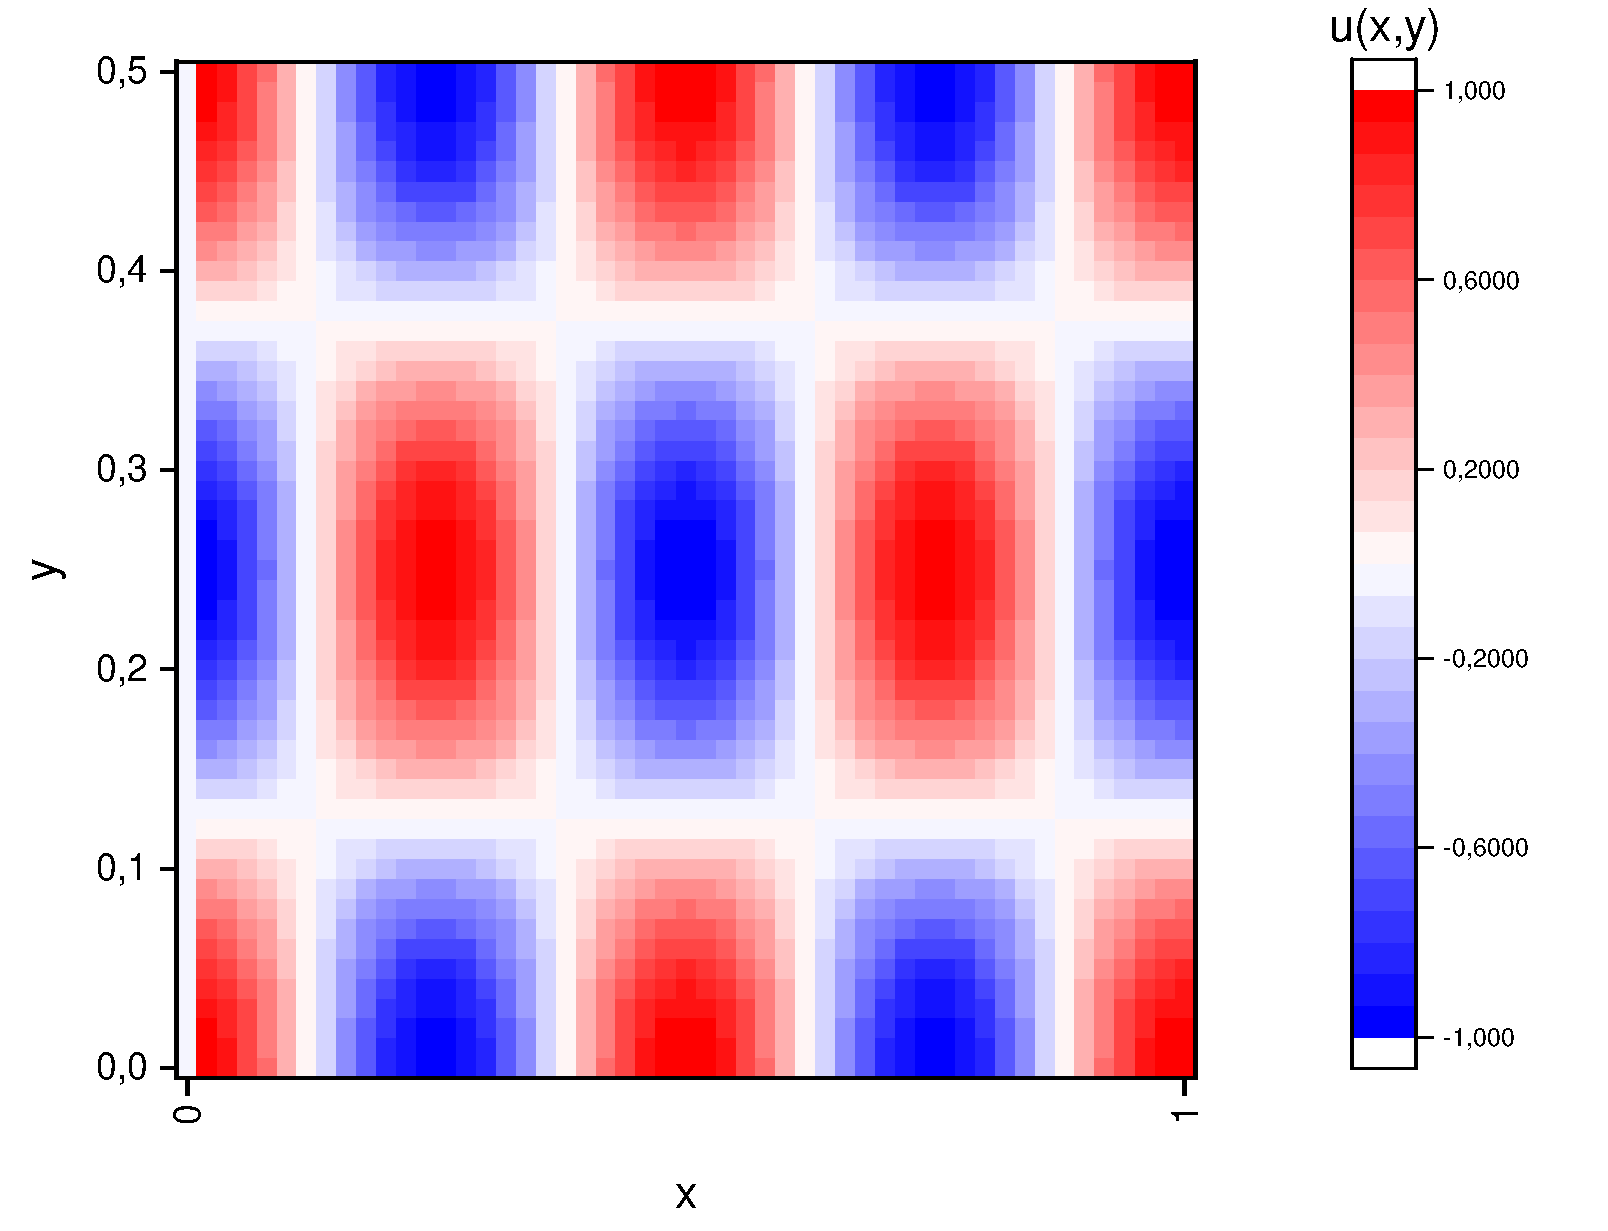
\includegraphics[scale=0.16]{graphs/graphs_a/v1/wave_t-0_v1.pdf} a
%	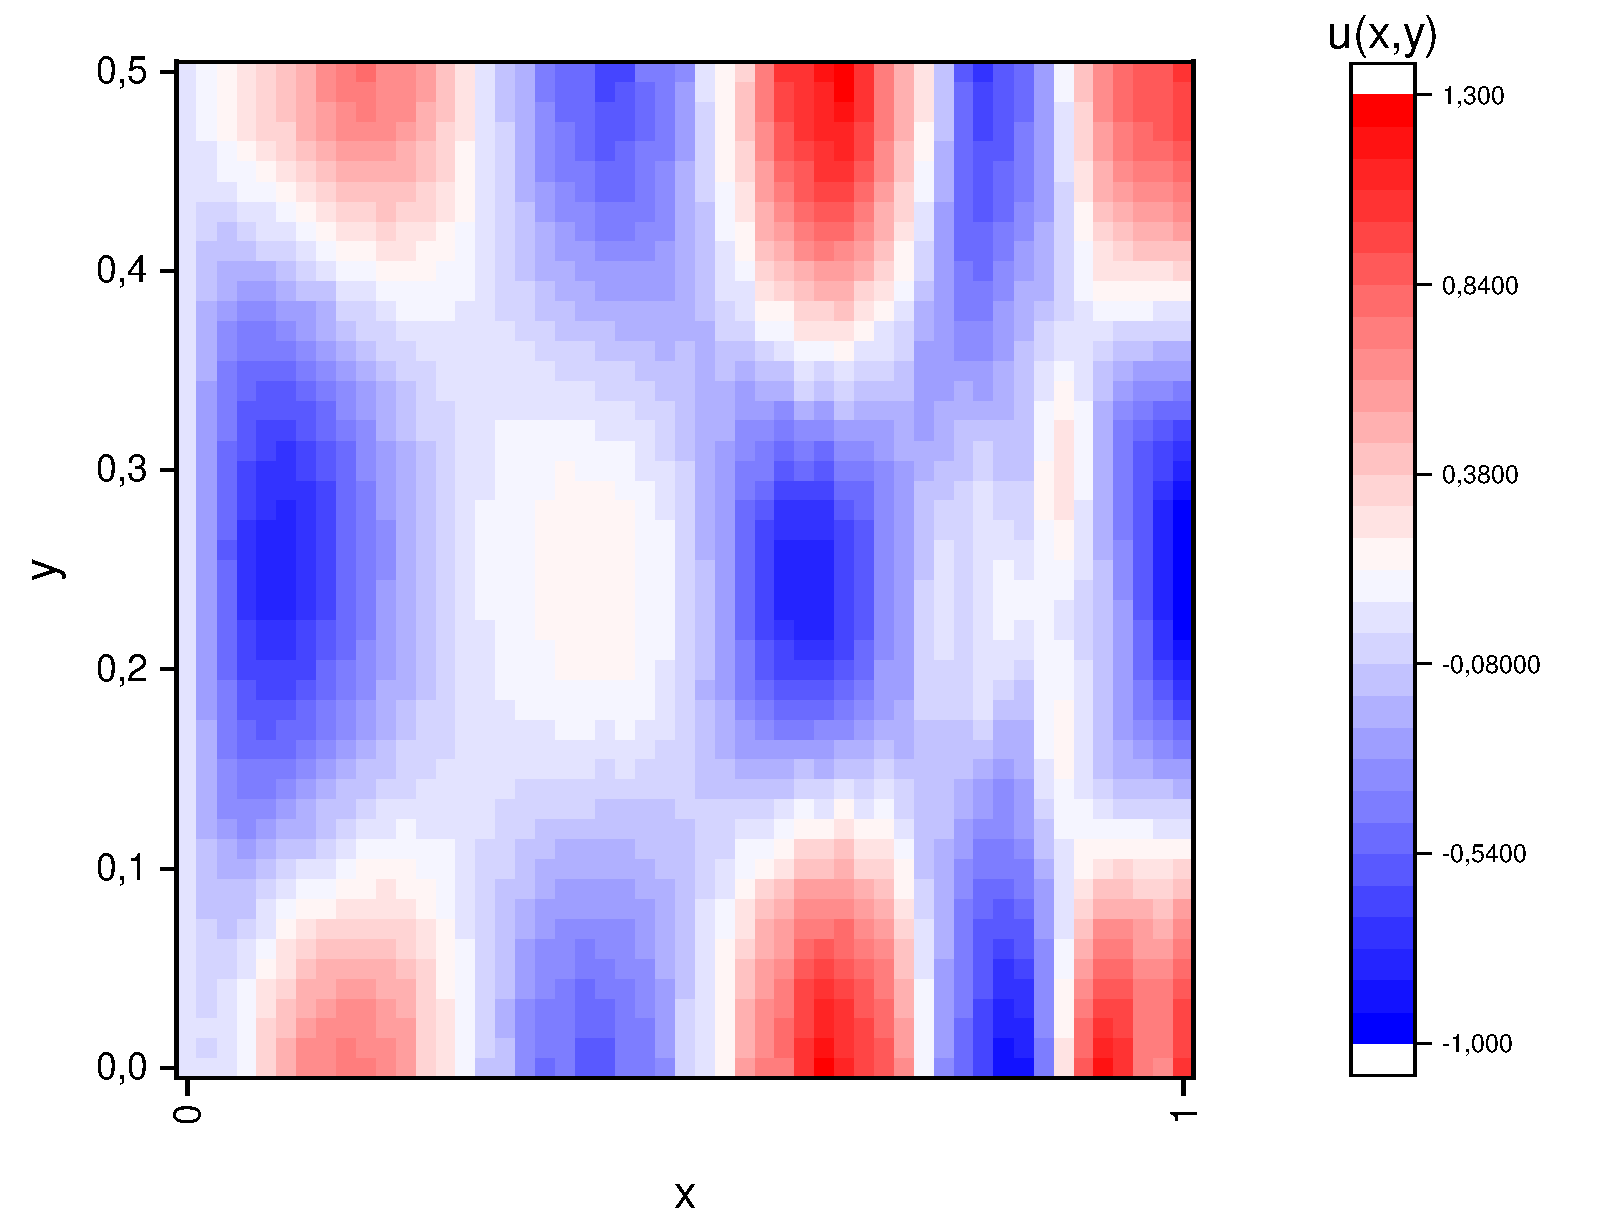
\includegraphics[scale=0.16]{graphs/graphs_a/v1/wave_t-6_v1.pdf} b
%	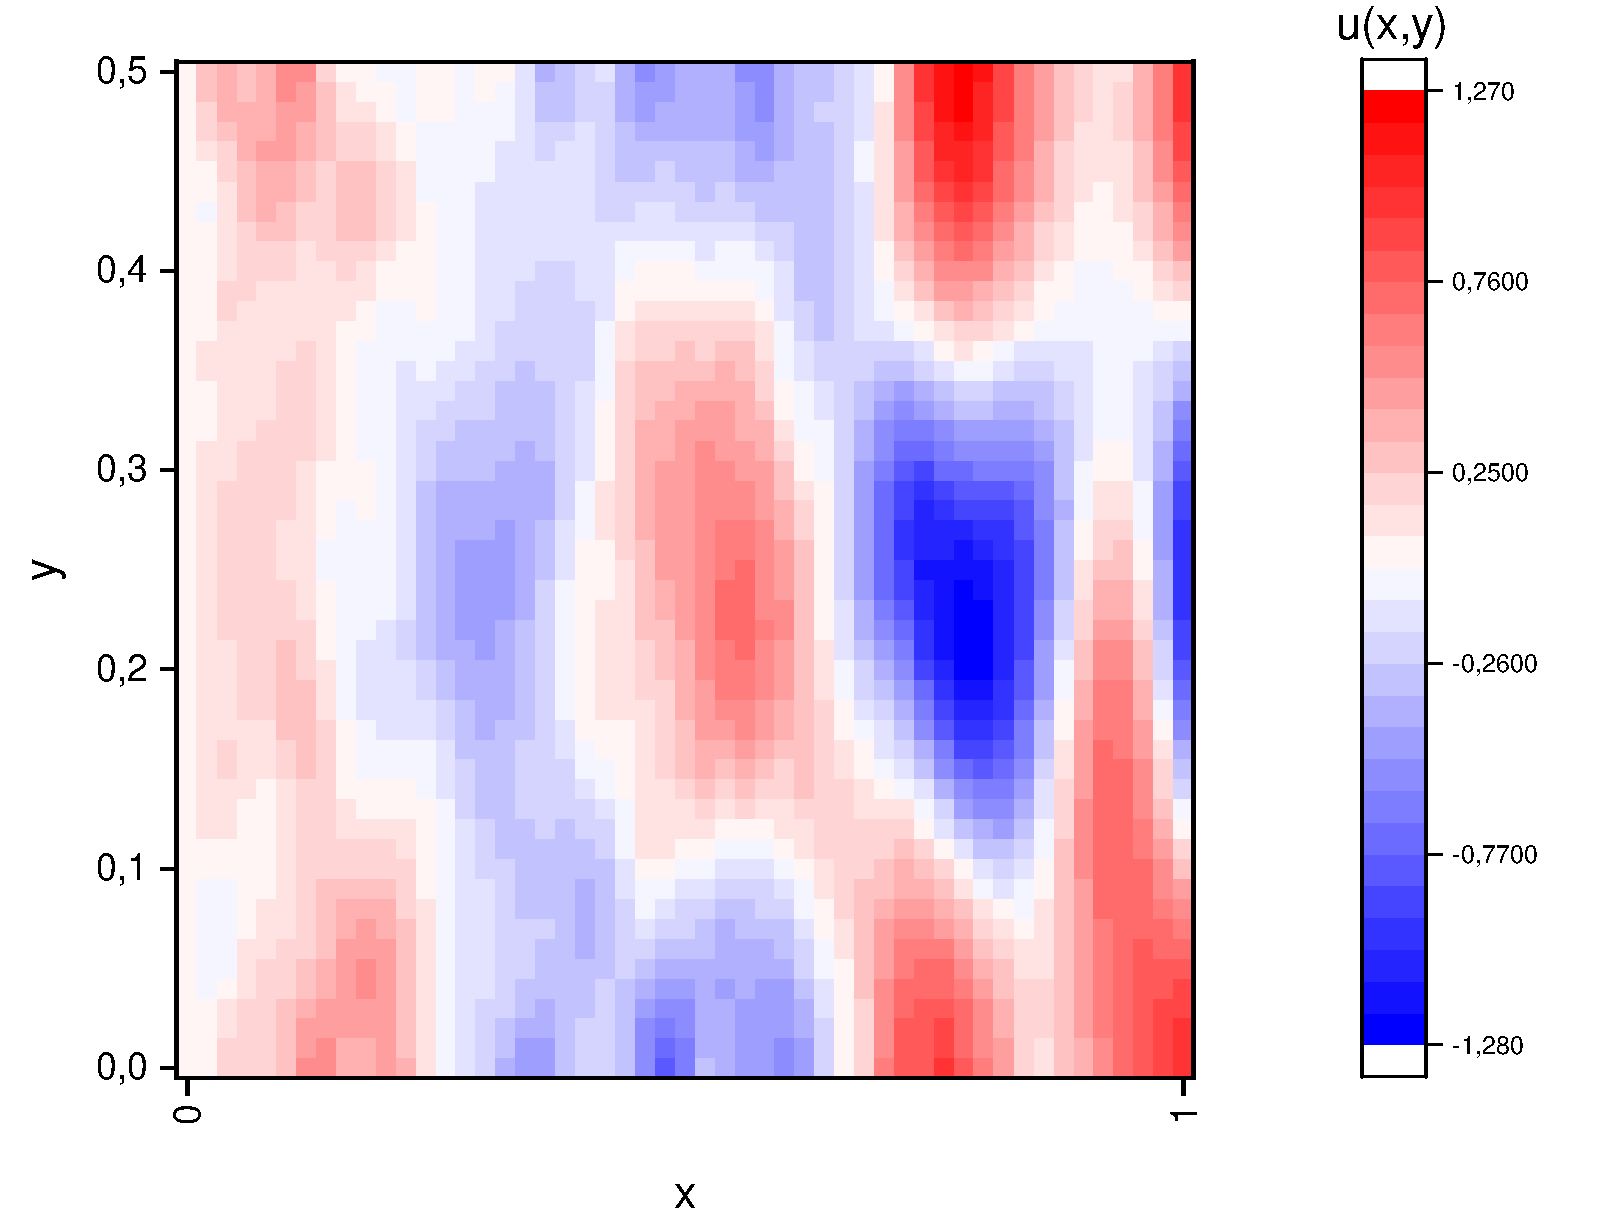
\includegraphics[scale=0.16]{graphs/graphs_a/v1/wave_t-16_v1.pdf} с
%	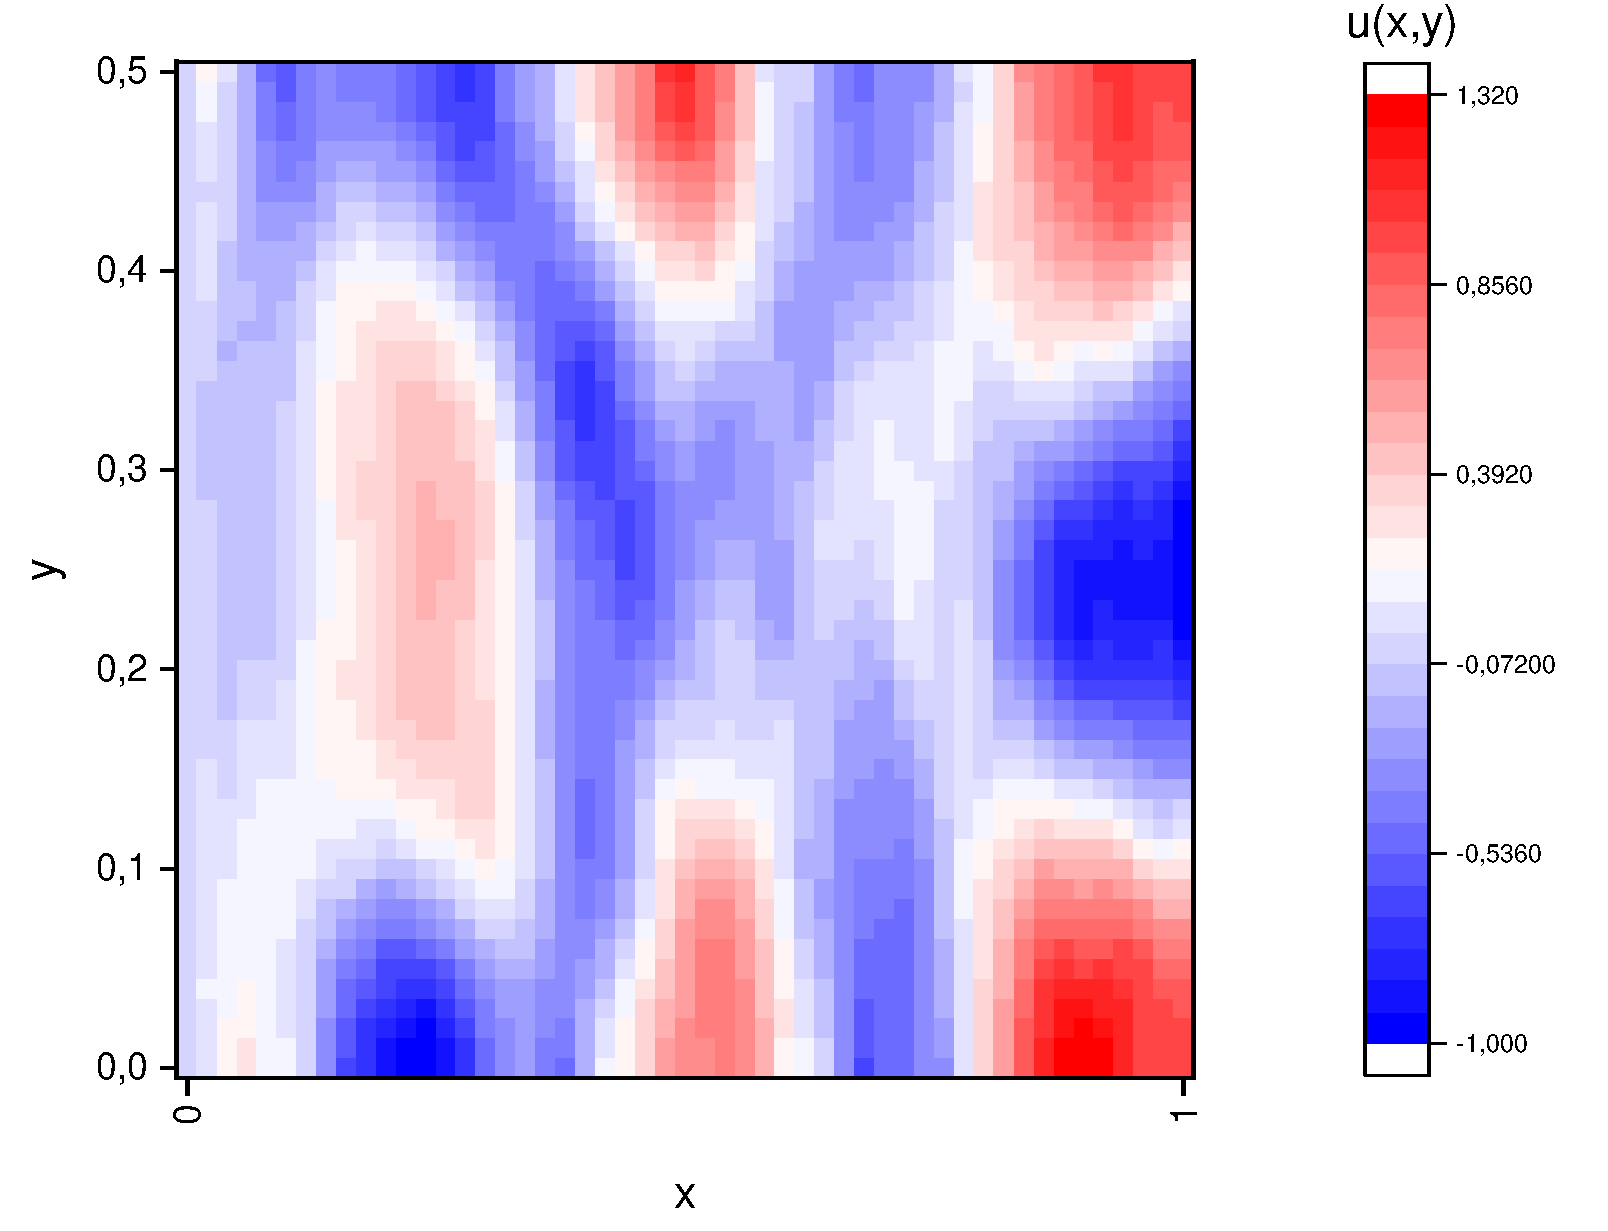
\includegraphics[scale=0.16]{graphs/graphs_a/v1/wave_t-24_v1.pdf} d
%	\caption{Решения}
%\end{figure}

\begin{figure}[h!]
	\begin{center}
		\begin{minipage}[h]{0.23\linewidth}
			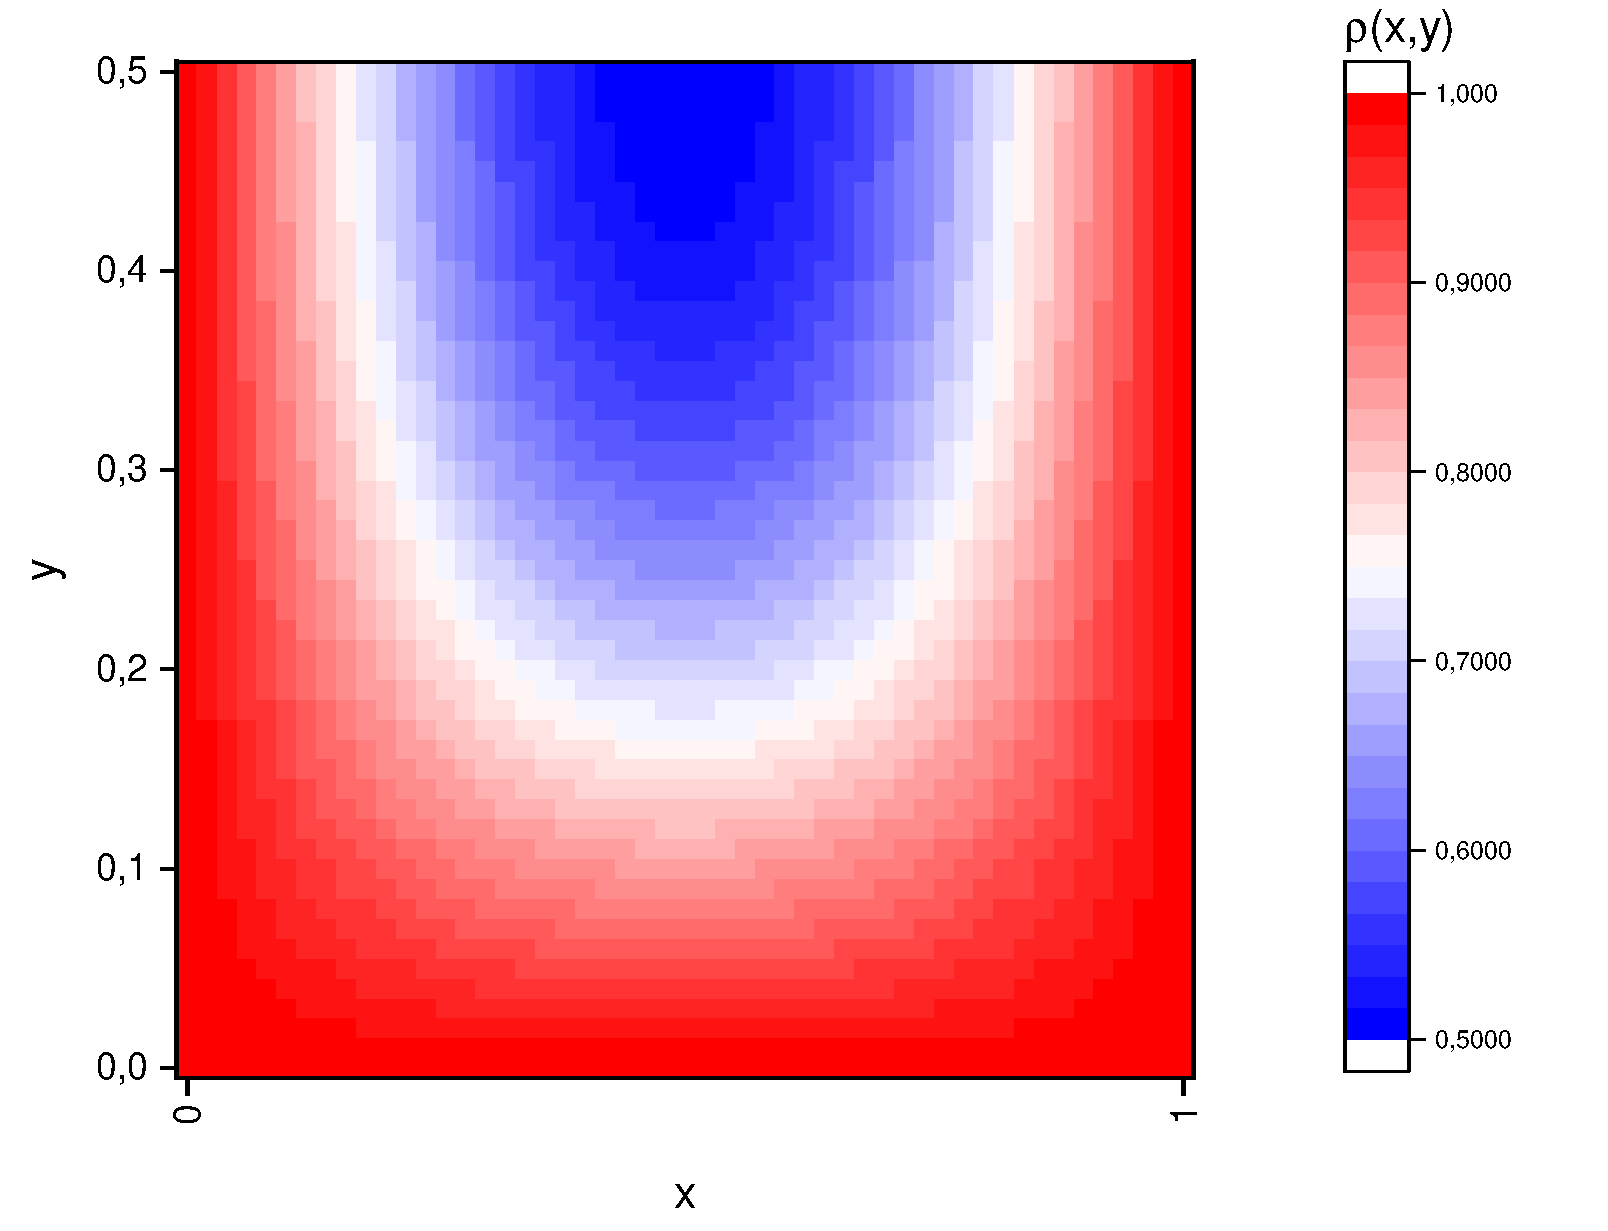
\includegraphics[width=\textwidth]{graphs/graphs_l/ro.pdf} \begin{center}	a)	\end{center}
		\end{minipage}
		\begin{minipage}[h]{0.23\linewidth}
			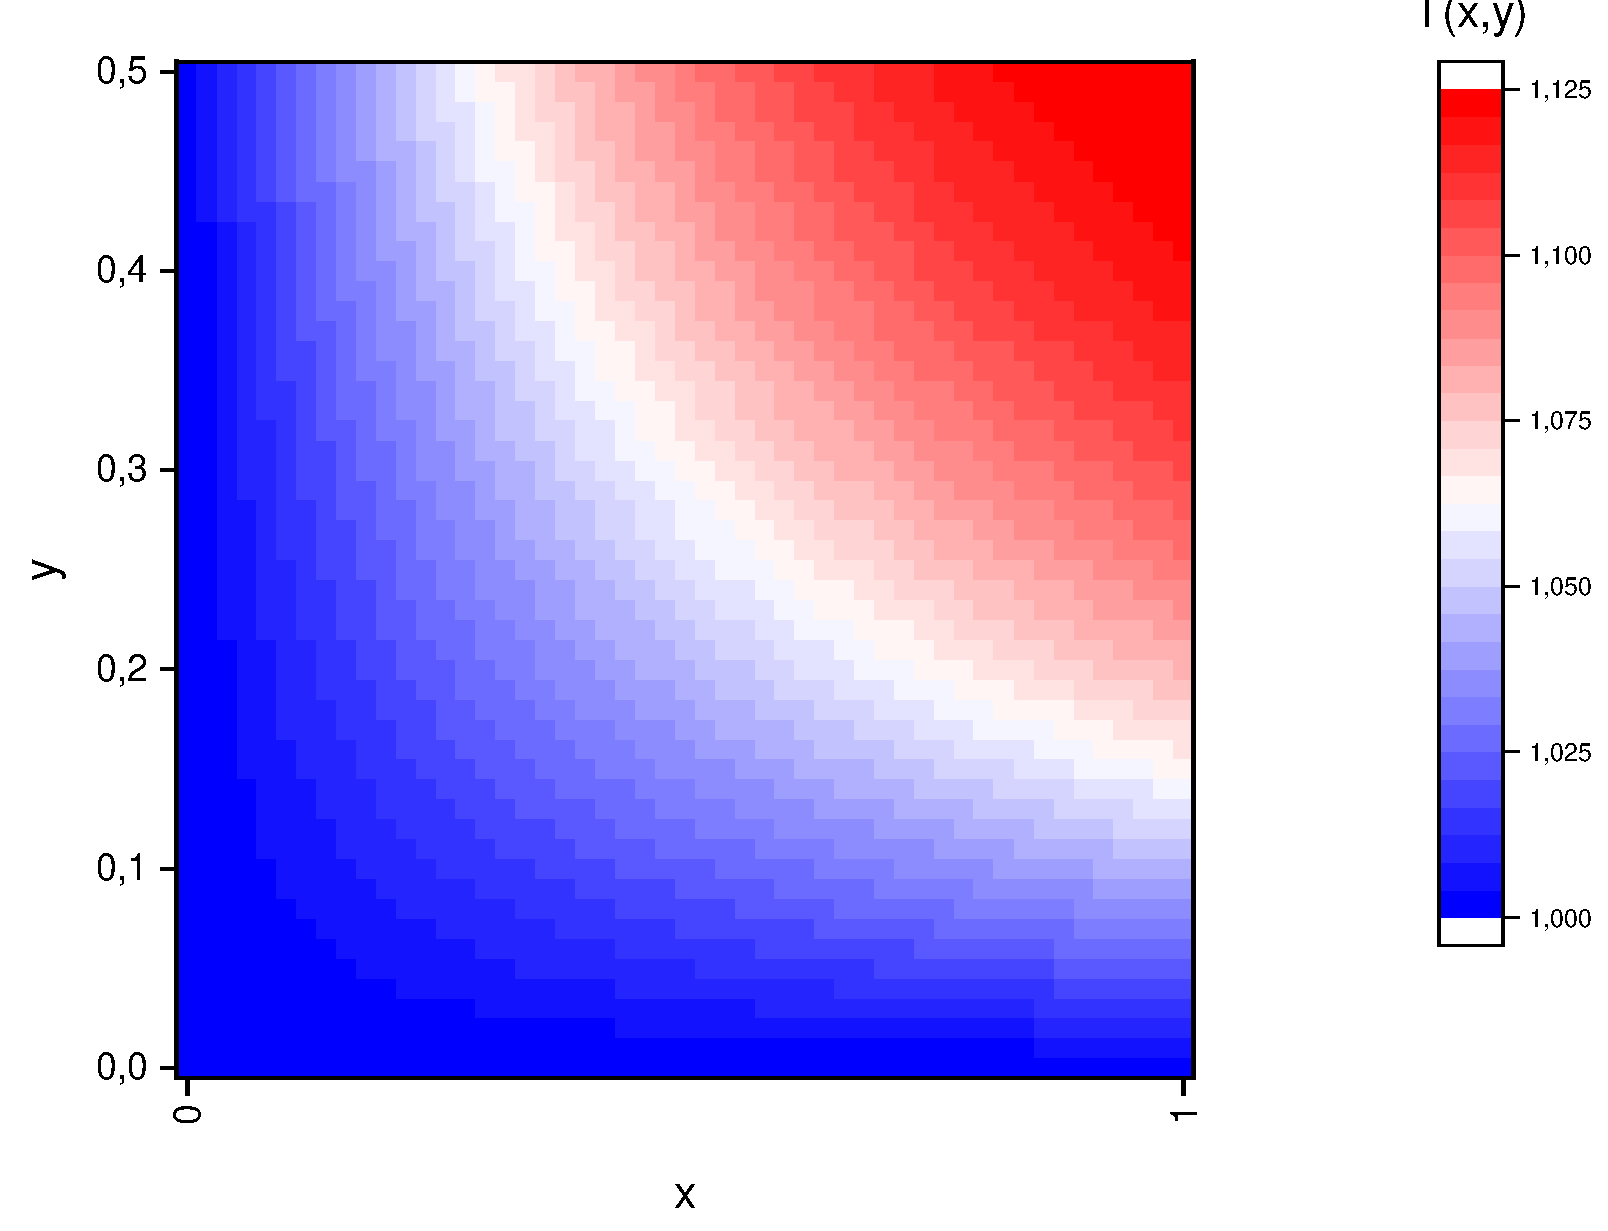
\includegraphics[width=\textwidth]{graphs/graphs_l/T.pdf} \begin{center}	c)	\end{center}
		\end{minipage}
		\begin{minipage}[h]{0.24\linewidth}
			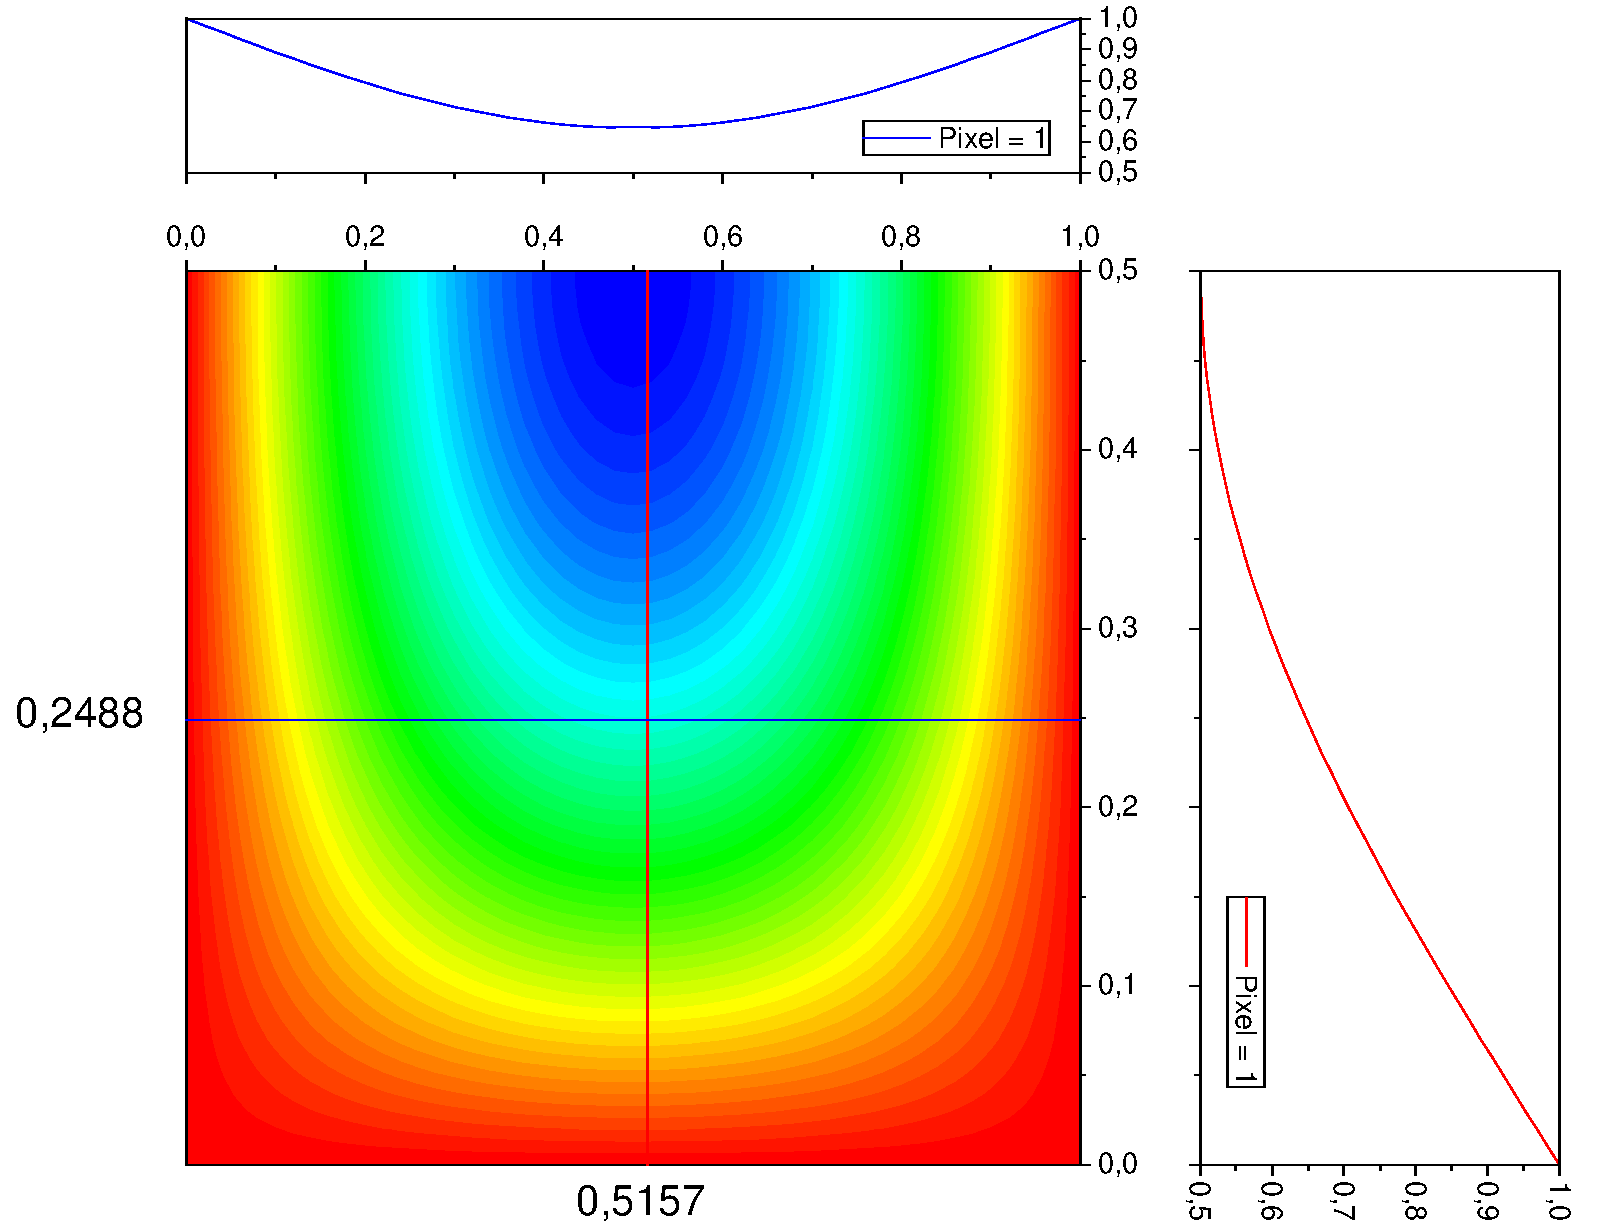
\includegraphics[width=\textwidth]{graphs/graphs_l/ro_srez.pdf} \begin{center}	b)	\end{center}
		\end{minipage}
		\begin{minipage}[h]{0.24\linewidth}
			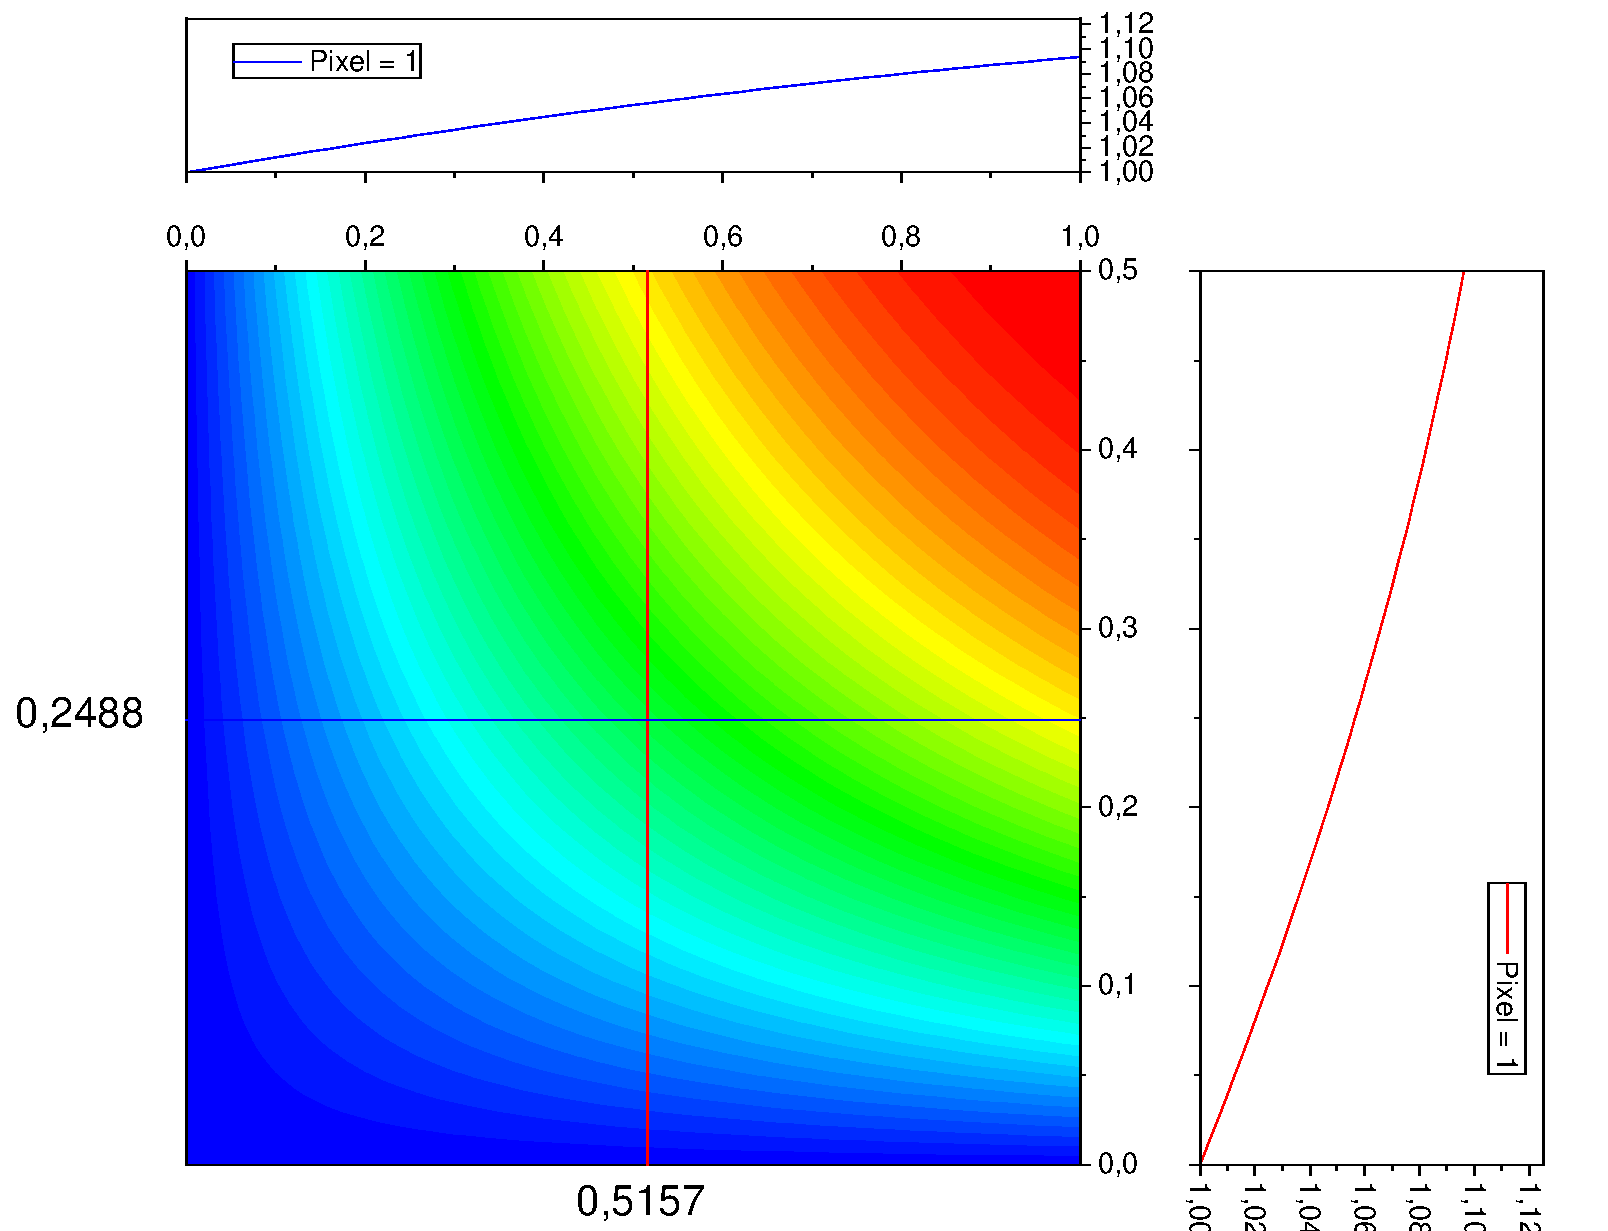
\includegraphics[width=\textwidth]{graphs/graphs_l/T_srez.pdf} \begin{center}	d)	\end{center}
		\end{minipage}
	\end{center}
	\caption{(a,b) График для $\lambda$ и его срез; (c,d) График для $c$ и его срез}
\end{figure}
%%%%%%%%%%%%%%%%%%%%%%%%%%%%%%%%%%%%%%%%%%%%%%%%%%%%%%%%%%%%%%%%%%%%%%%%%%%
Варианты графиков v1
\begin{figure}[h!]
	\begin{center}
		\begin{minipage}[h]{0.23\linewidth}
			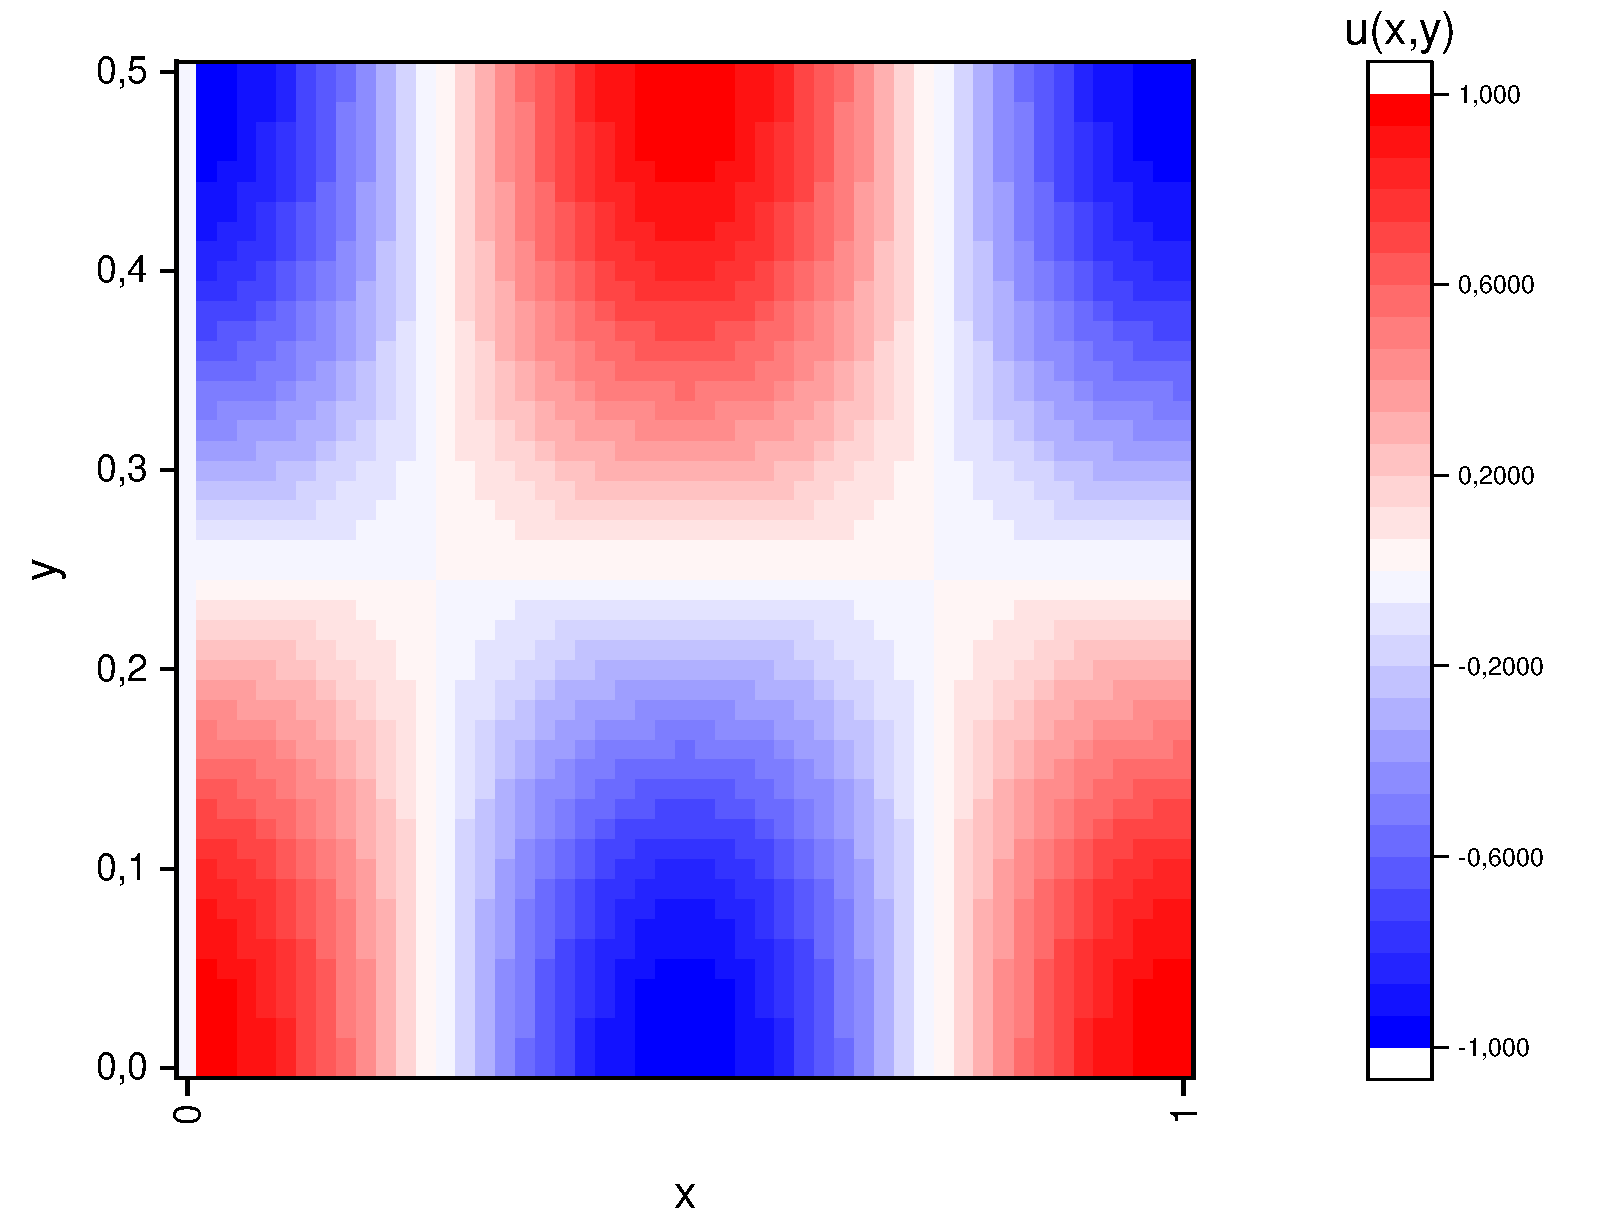
\includegraphics[width=\textwidth]{graphs/graphs_l/v1/wave_t-0_v1.pdf} \begin{center}	a)	\end{center}
		\end{minipage}
		\begin{minipage}[h]{0.23\linewidth}
			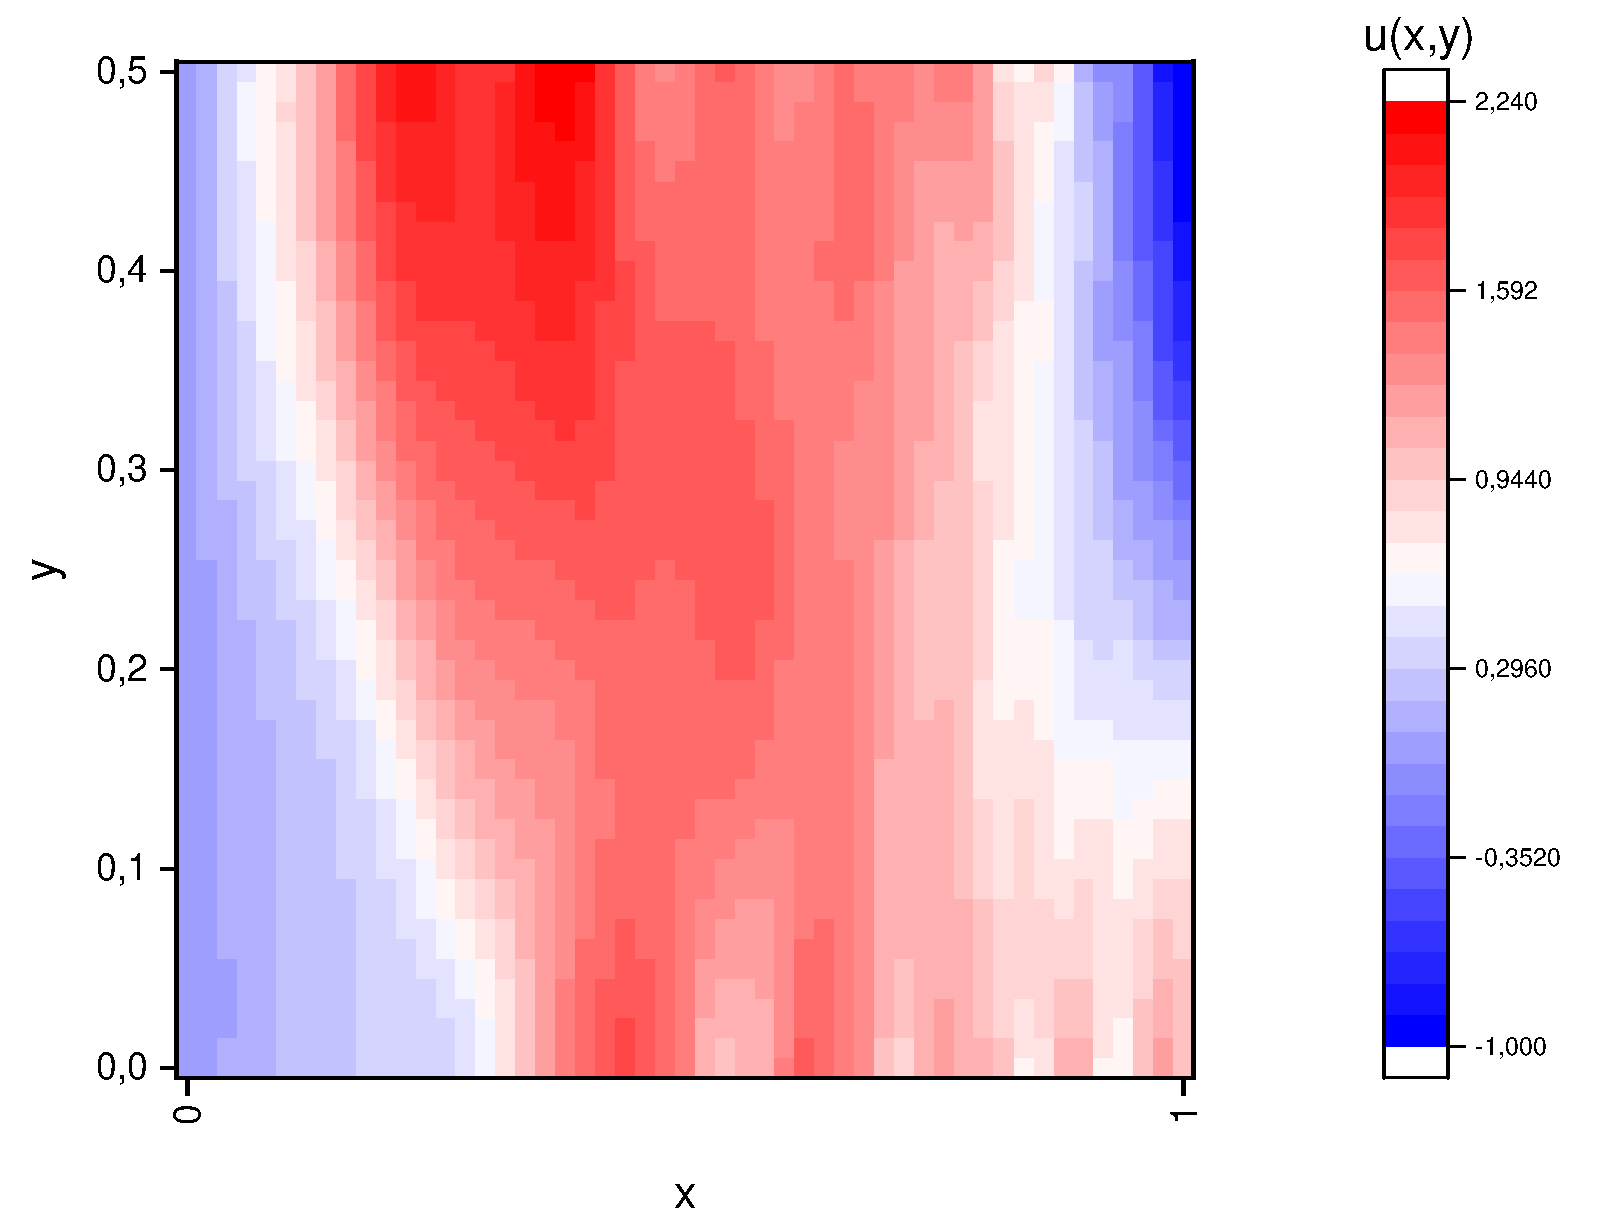
\includegraphics[width=\textwidth]{graphs/graphs_l/v1/wave_t-8_v1.pdf} \begin{center}	b)	\end{center}
		\end{minipage}
		\begin{minipage}[h]{0.23\linewidth}
			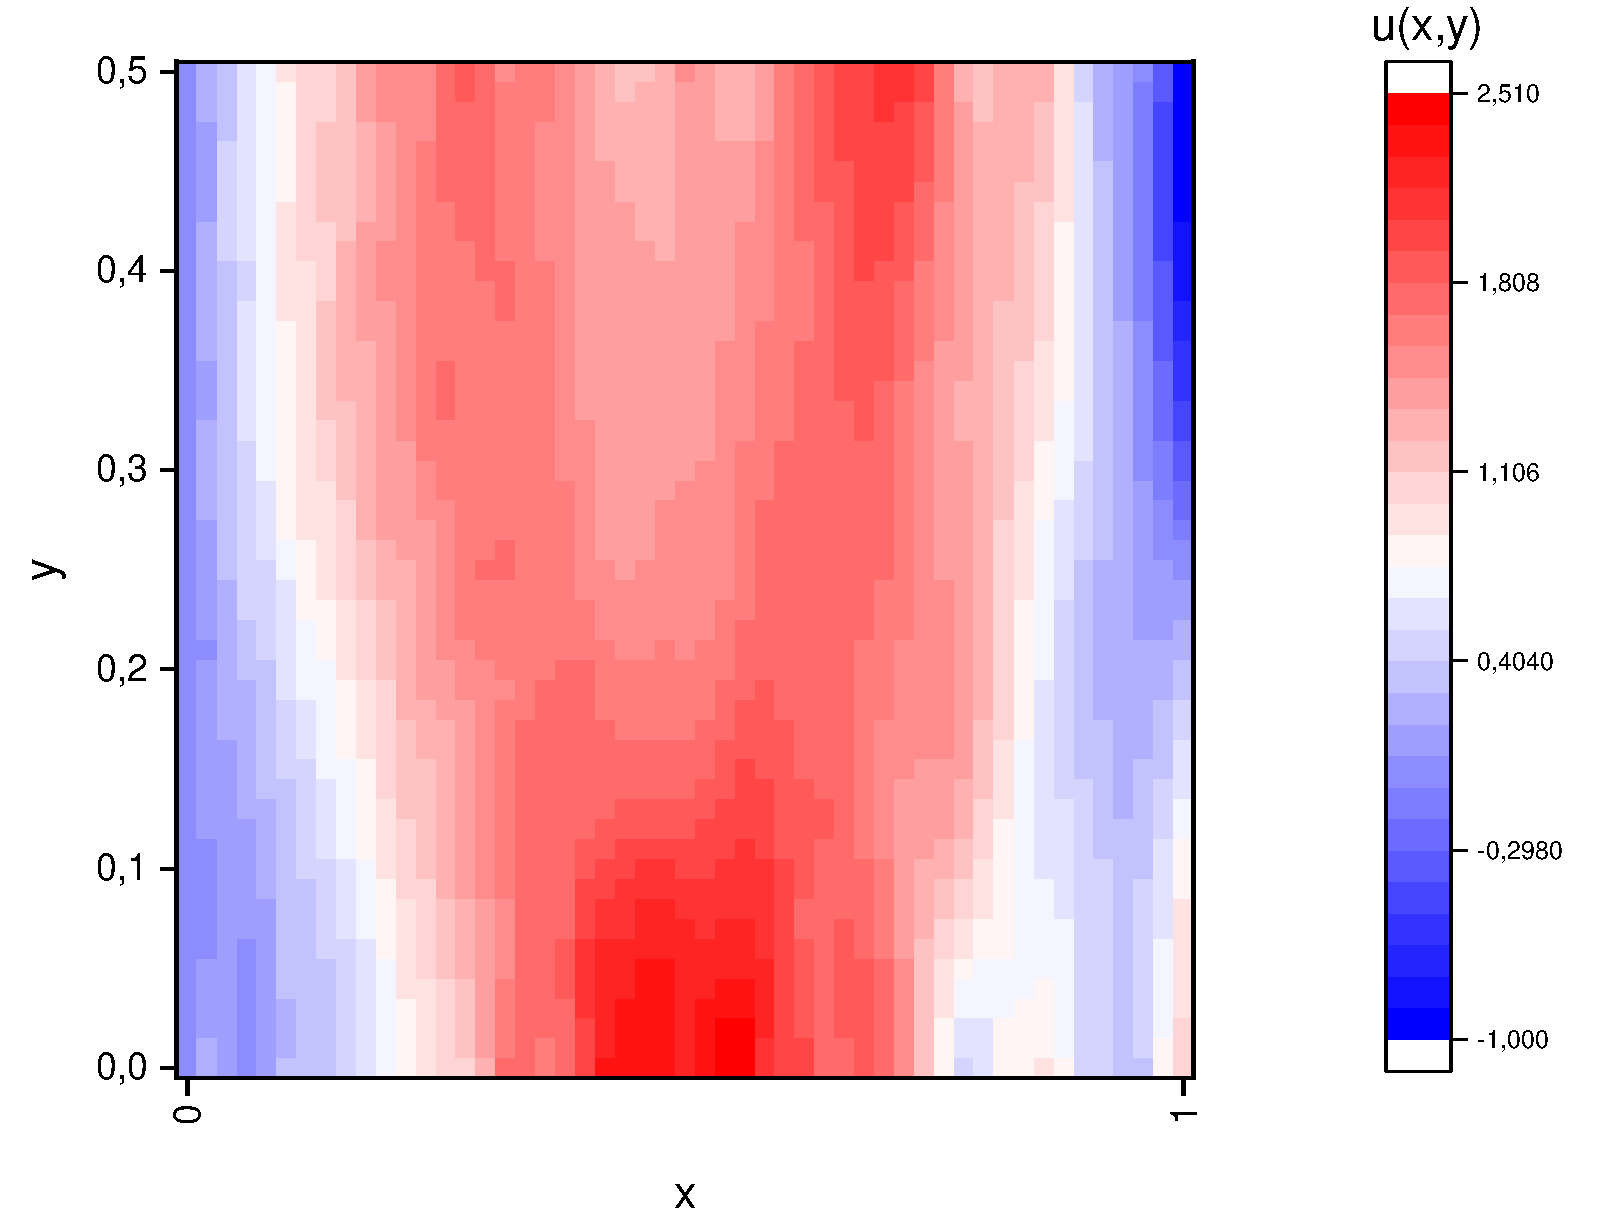
\includegraphics[width=\textwidth]{graphs/graphs_l/v1/wave_t-16_v1.pdf} \begin{center}	c)	\end{center}
		\end{minipage}
		\begin{minipage}[h]{0.23\linewidth}
			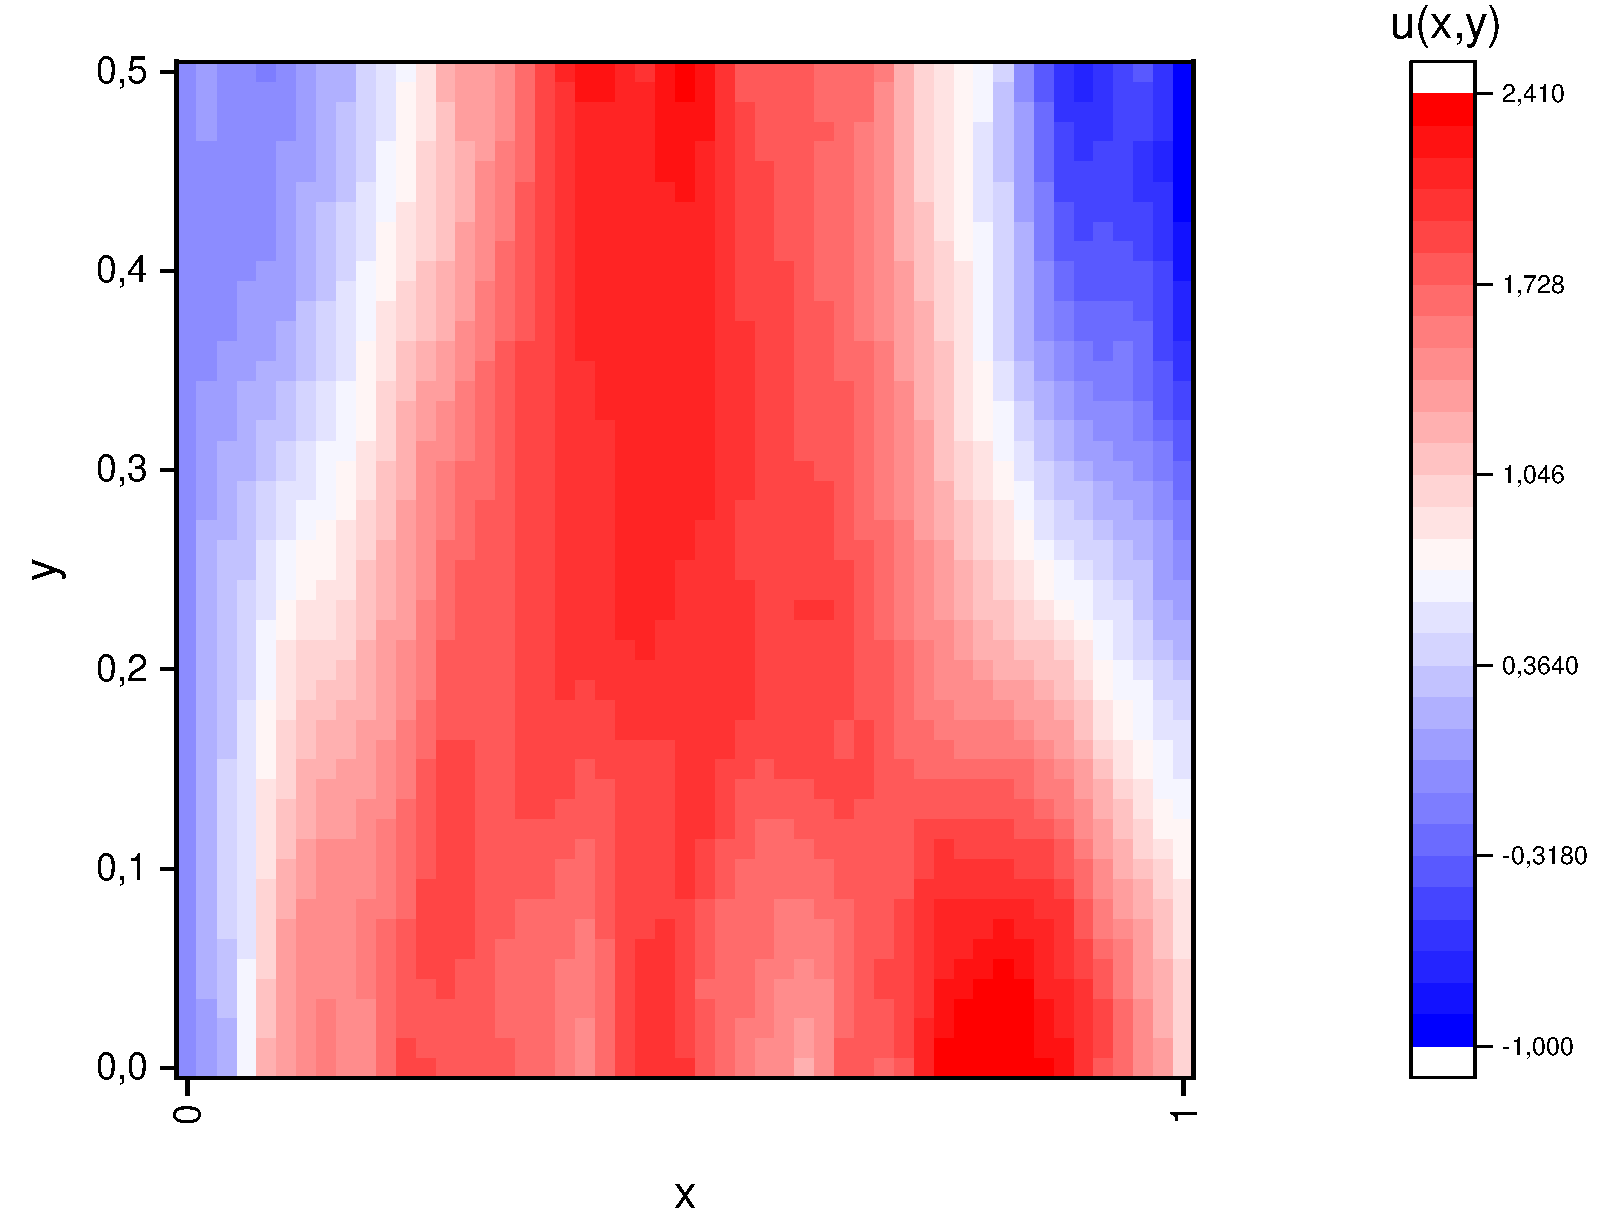
\includegraphics[width=\textwidth]{graphs/graphs_l/v1/wave_t-24_v1.pdf} \begin{center}	d)	\end{center}
		\end{minipage}
	\end{center}
	\caption{Решение для моментов времени (a)$\ t = 0.0$, (b) $\ t = 1.6$, (c)$\ t = 3.2$, (	d)$\ t = 4.8$.}
\end{figure}

Варианты графиков v1 srez
\begin{figure}[h!]
	\begin{center}
		\begin{minipage}[h]{0.24\linewidth}
			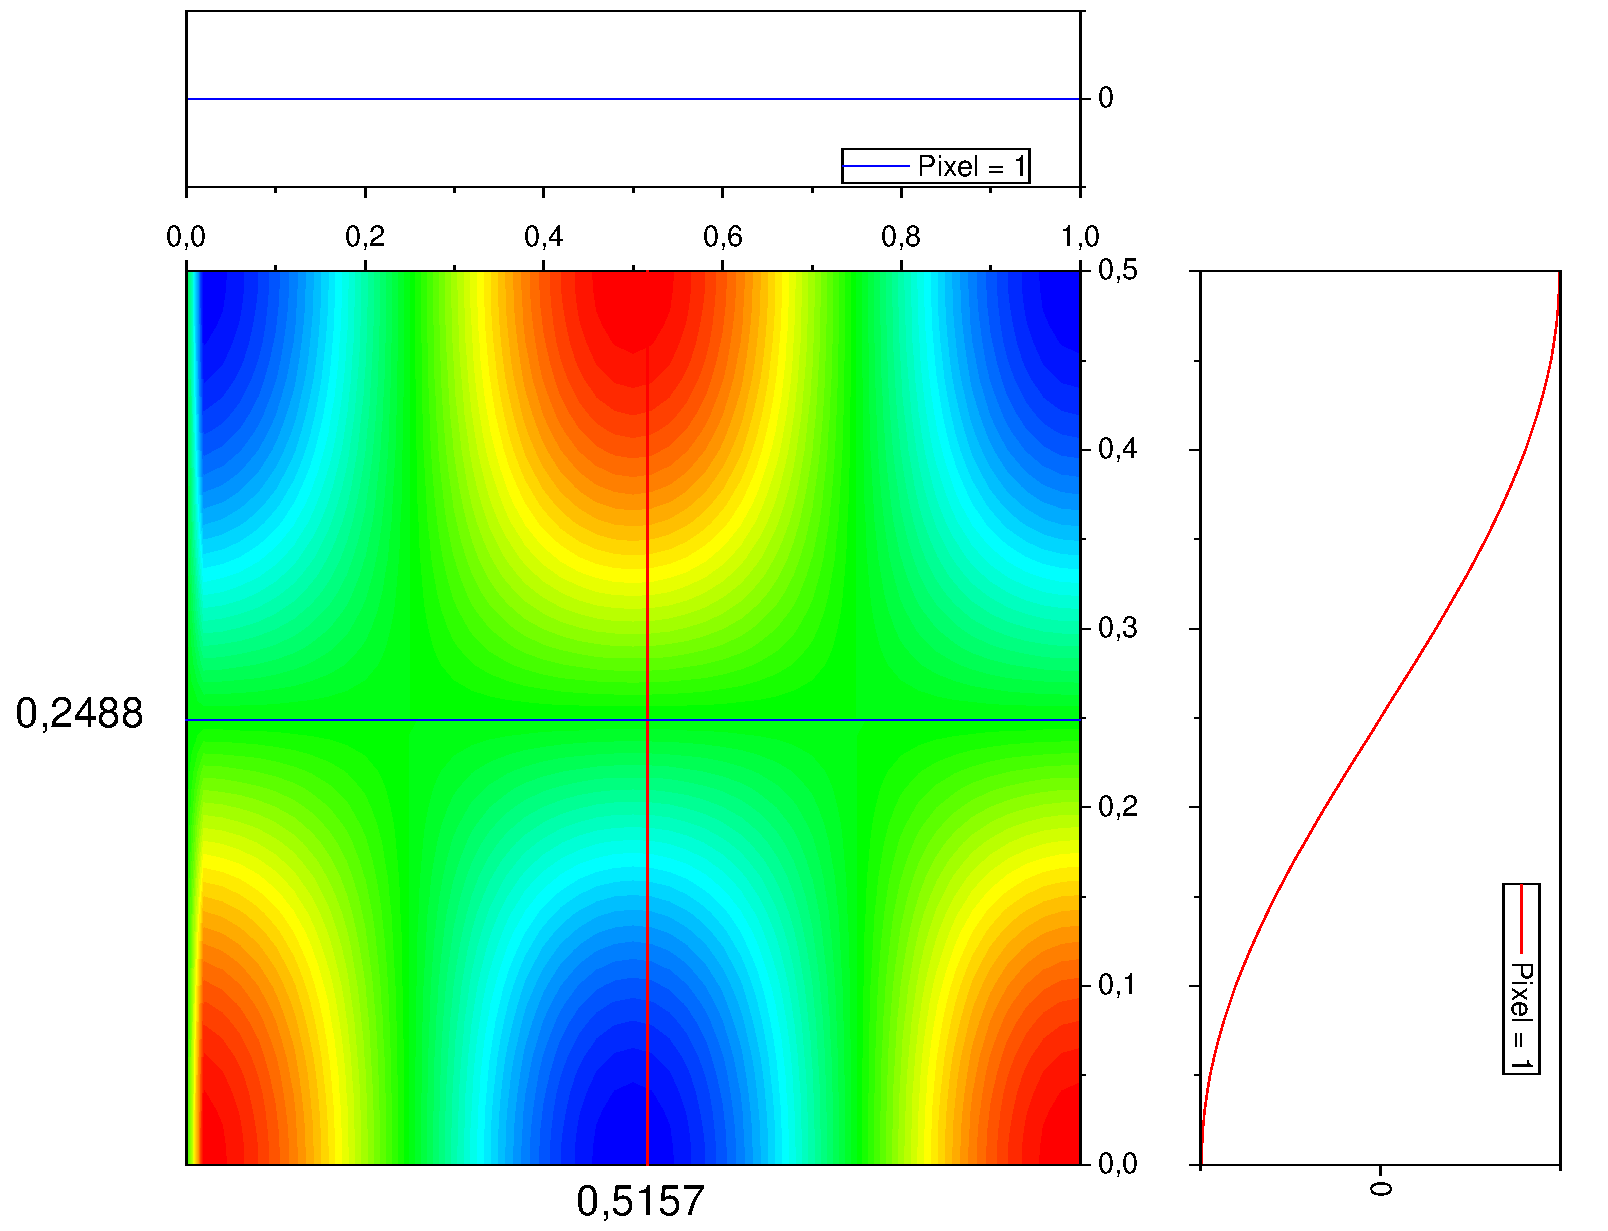
\includegraphics[width=\textwidth]{graphs/graphs_l/v1/wave_t-0_v1_srez} \begin{center}	a)	\end{center}
		\end{minipage}
		\begin{minipage}[h]{0.24\linewidth}
			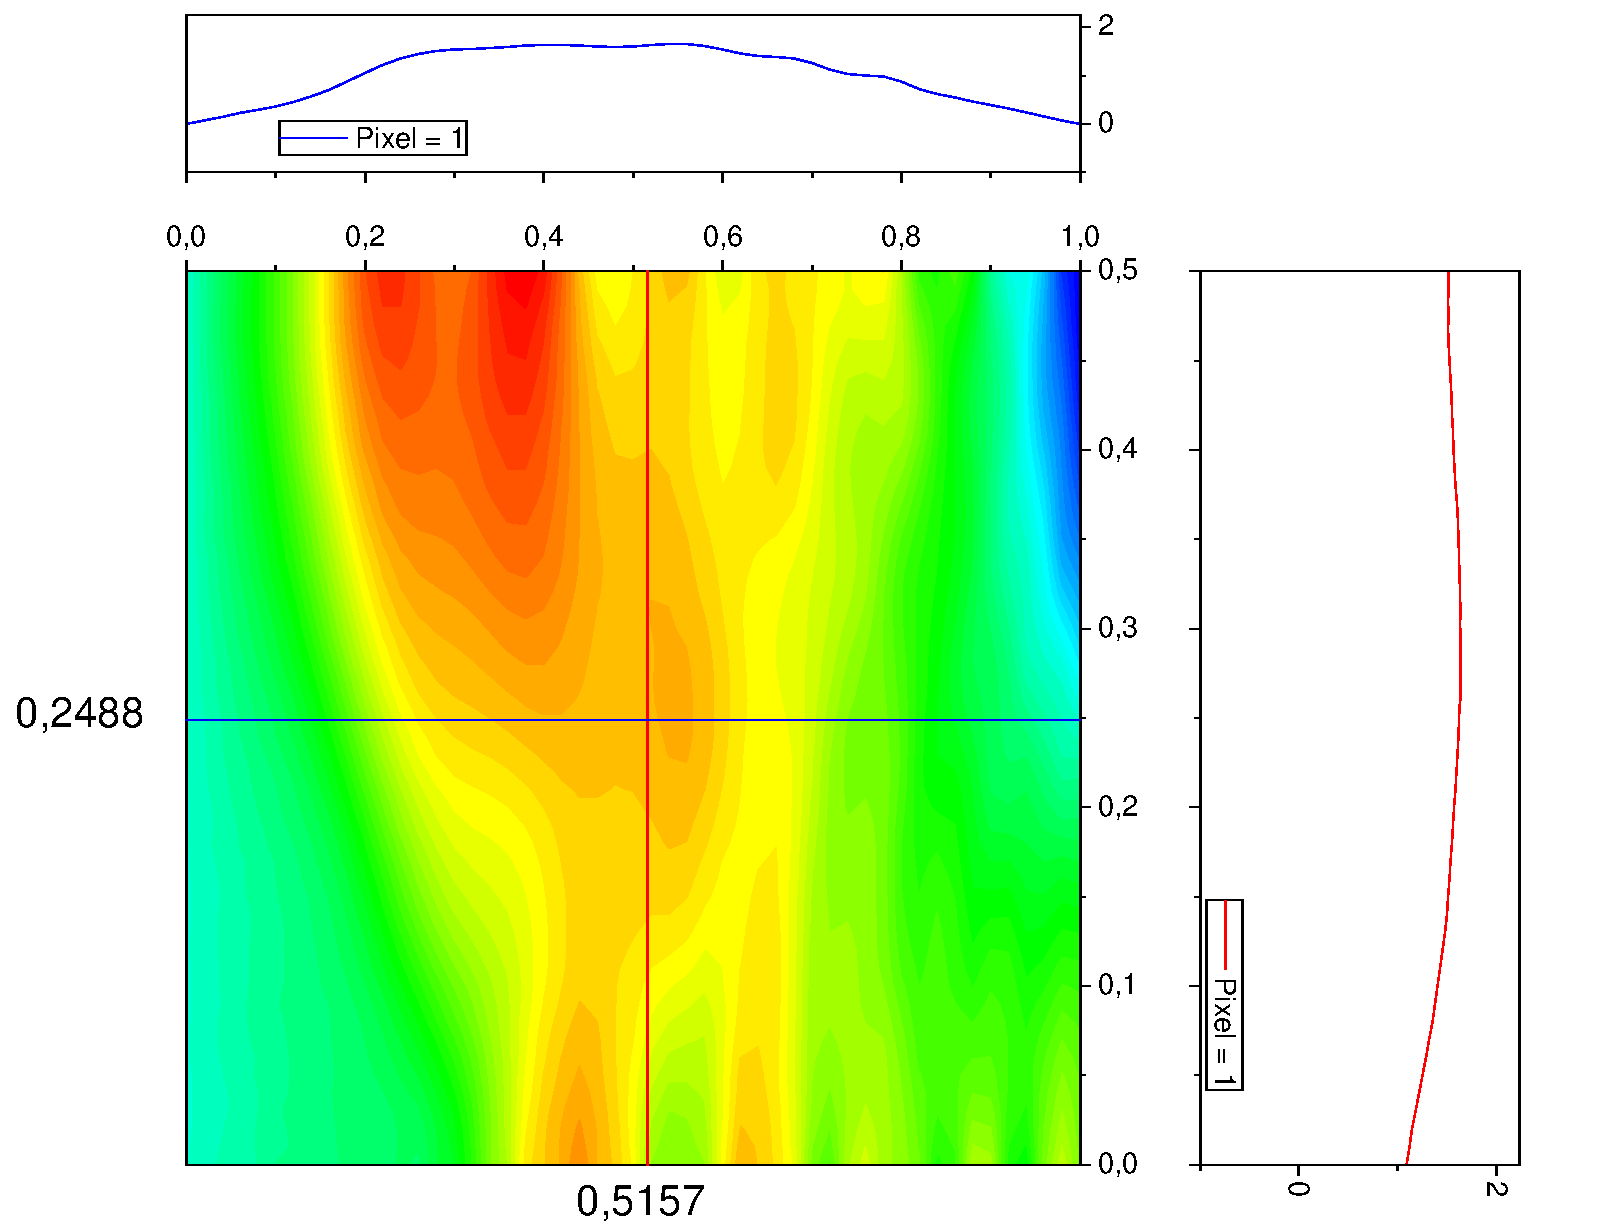
\includegraphics[width=\textwidth]{graphs/graphs_l/v1/wave_t-8_v1_srez} \begin{center}	b)	\end{center}
		\end{minipage}
		\begin{minipage}[h]{0.24\linewidth}
			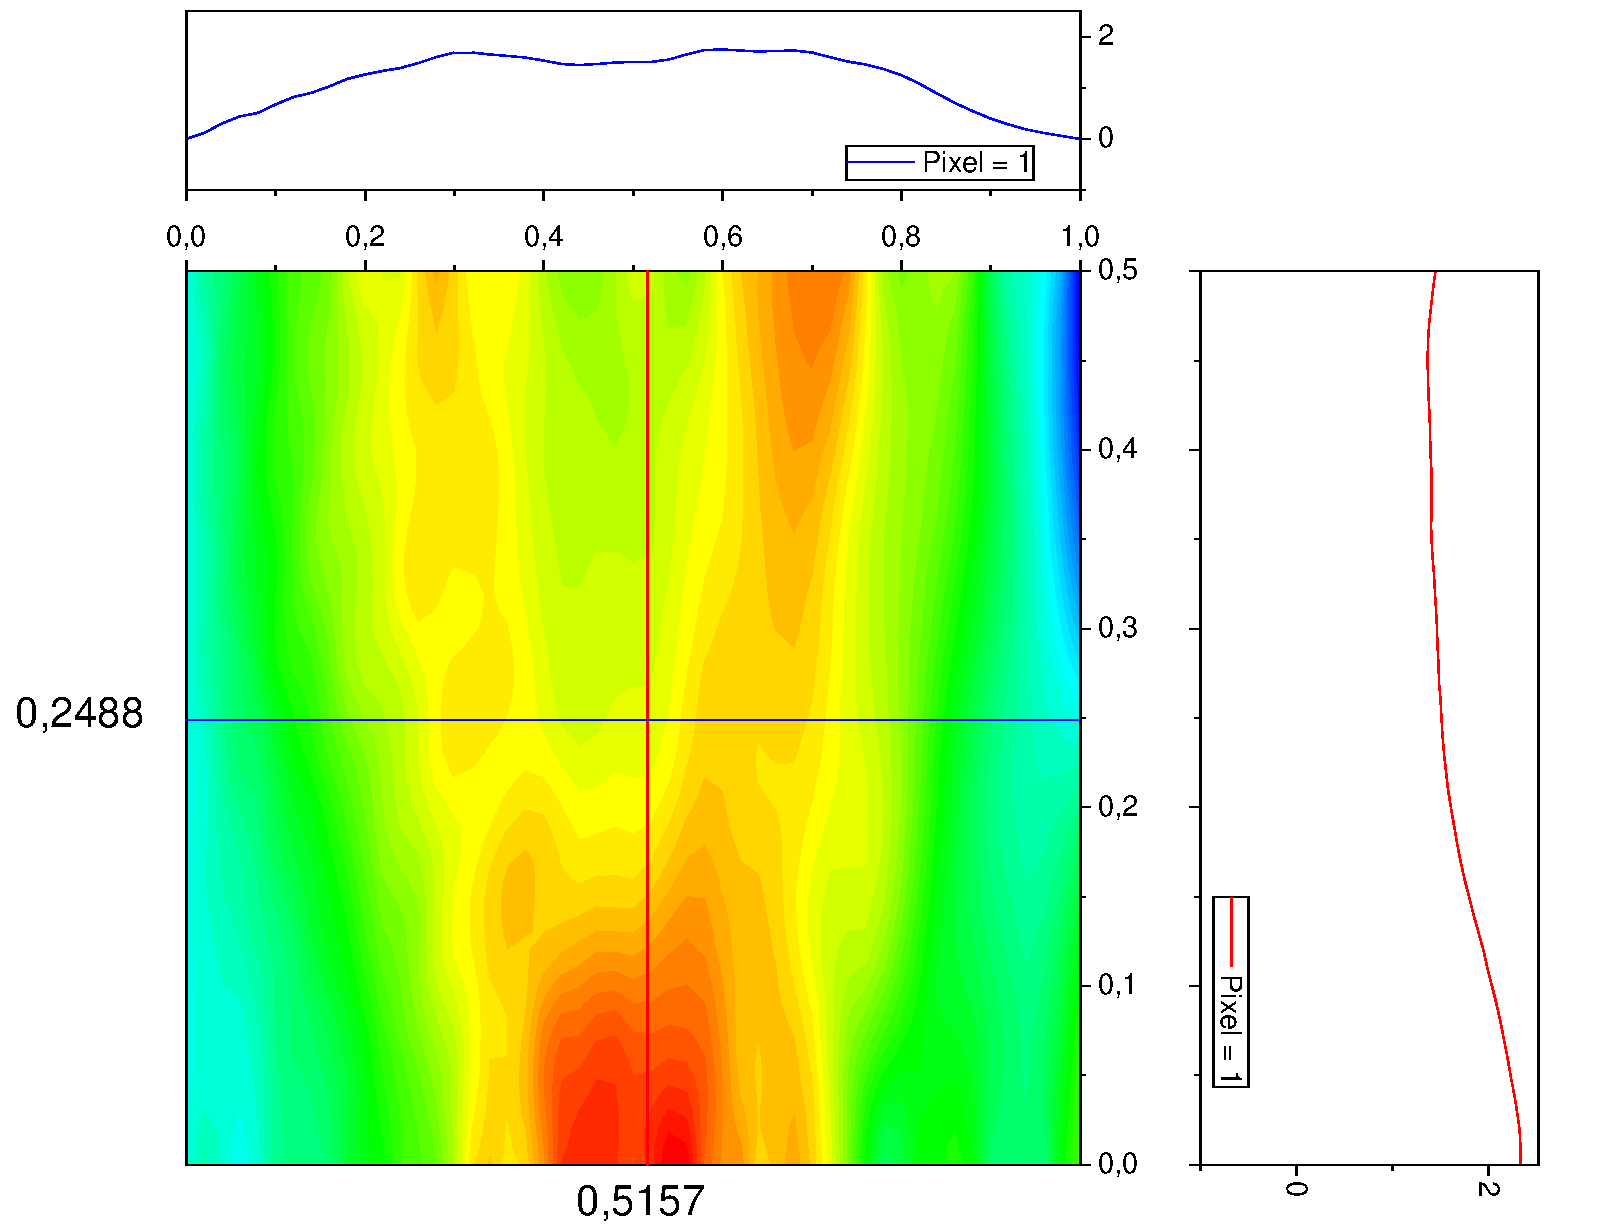
\includegraphics[width=\textwidth]{graphs/graphs_l/v1/wave_t-16_v1_srez} \begin{center}	c)	\end{center}
		\end{minipage}
		\begin{minipage}[h]{0.24\linewidth}
			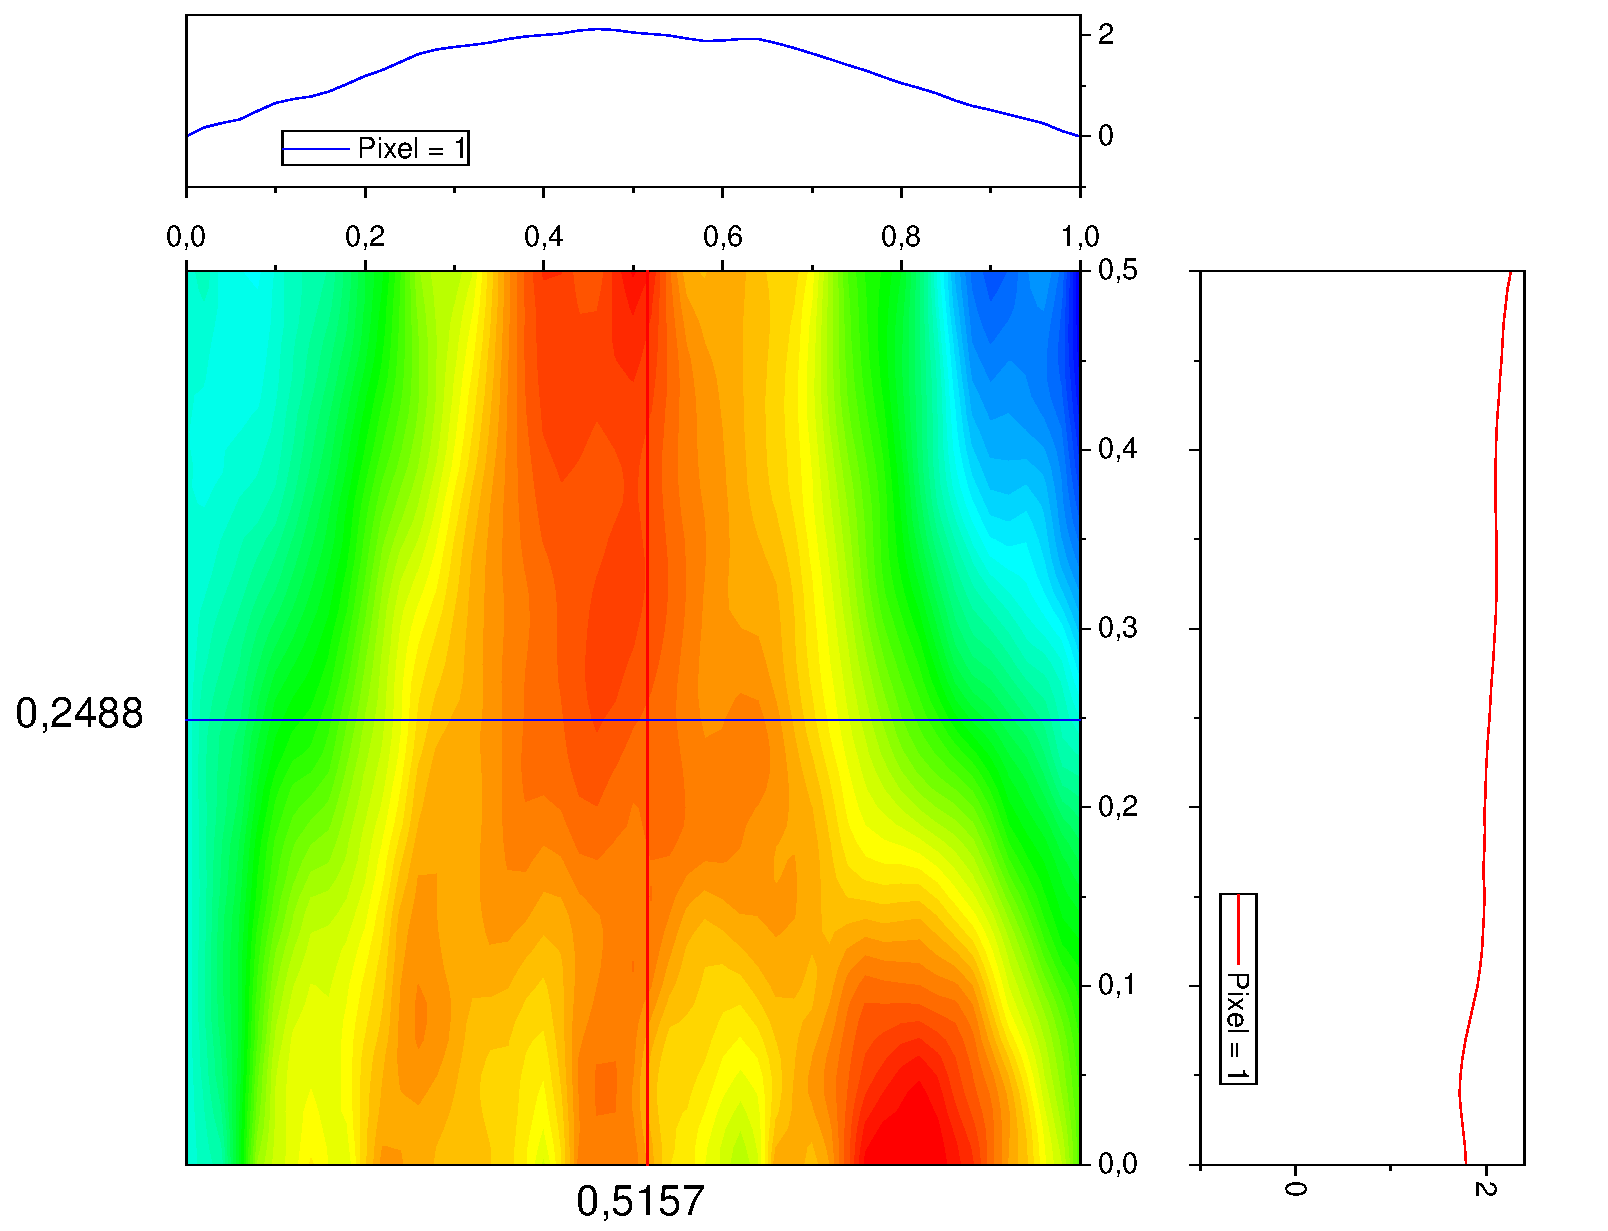
\includegraphics[width=\textwidth]{graphs/graphs_l/v1/wave_t-24_v1_srez} \begin{center}	d)	\end{center}
		\end{minipage}
	\end{center}
	\caption{Срезы решения для моментов времени (a)$\ t = 0.0$, (b) $\ t = 1.6$, (c)$\ t = 3.2$, (d)$\ t = 4.8$}
\end{figure}
%%%%%%%%%%%%%%%%%%%%%%%%%%%%%%%%%%%%%%%%%%%%%%%%%%%%%%%%%%%%%%%%%%%%%%%%%%%
Варианты графиков v2
\begin{figure}[h!]
	\begin{center}
		\begin{minipage}[h]{0.23\linewidth}
			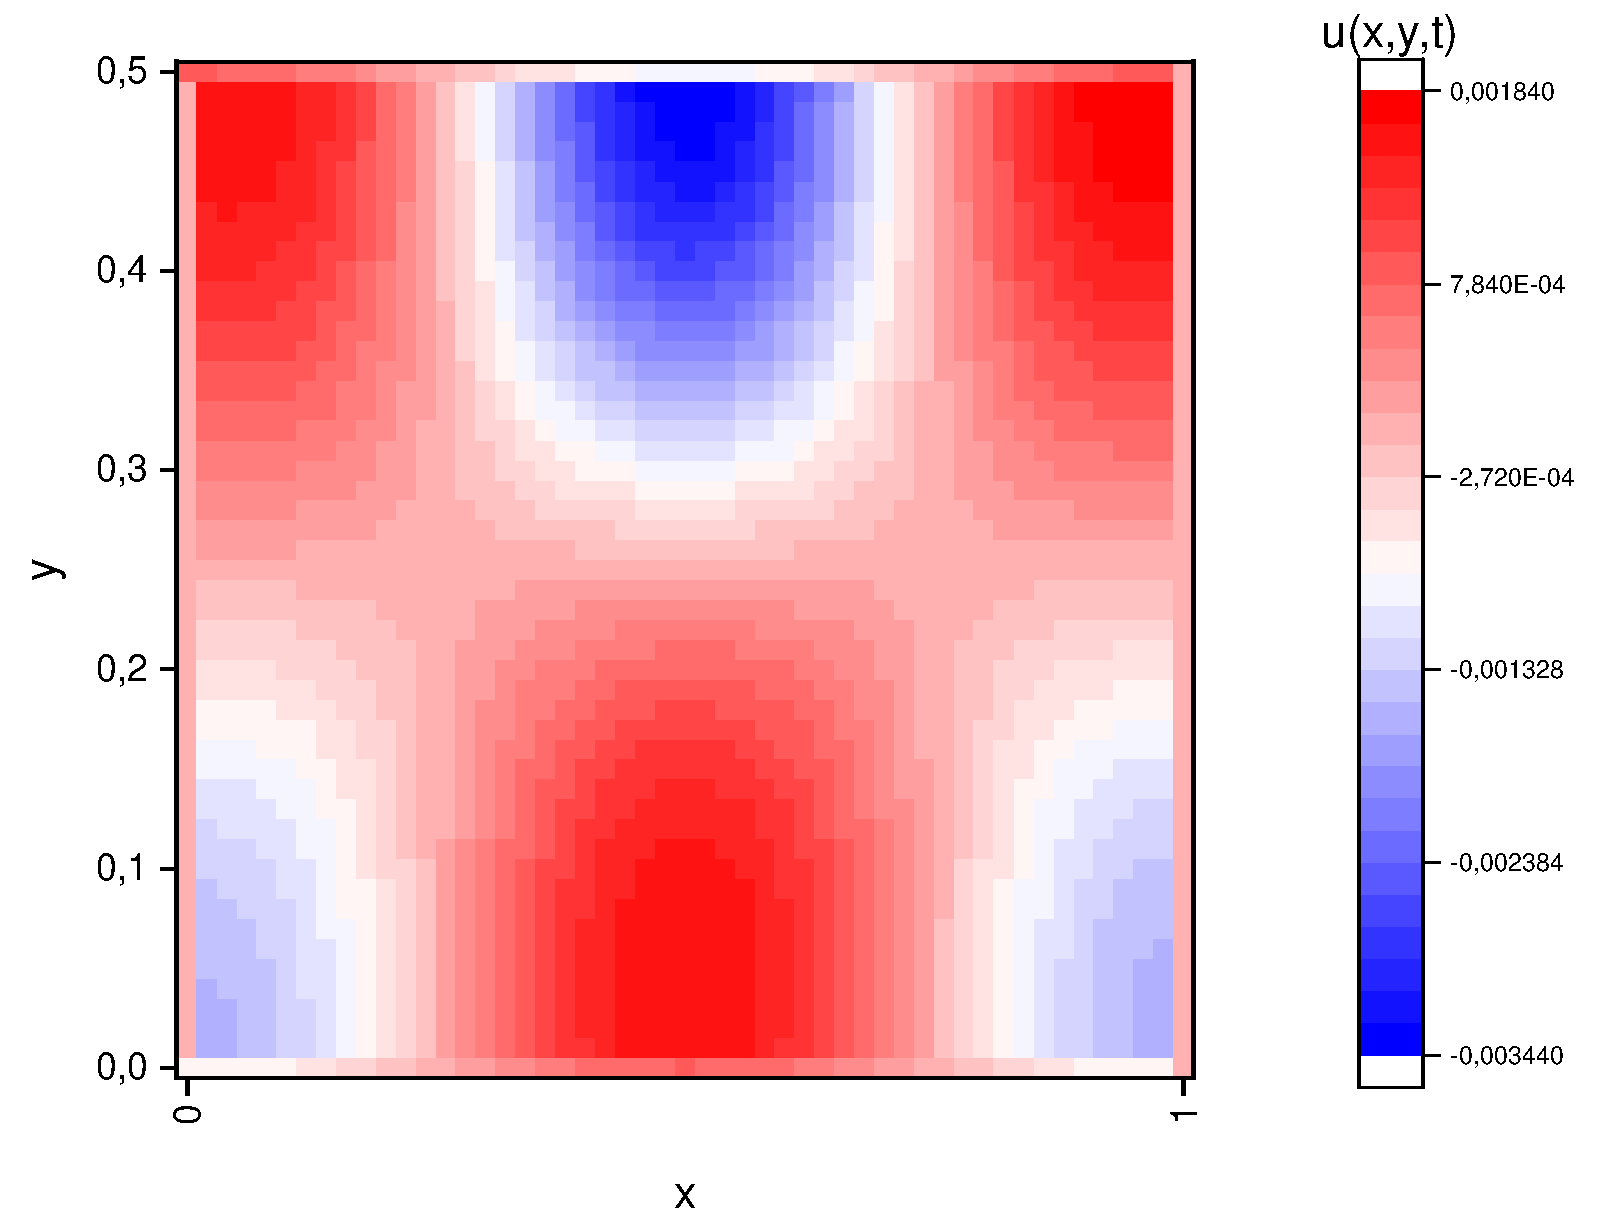
\includegraphics[width=\textwidth]{graphs/graphs_l/v2/wave_t-0_v2.pdf} \begin{center}	a)	\end{center}
		\end{minipage}
		\begin{minipage}[h]{0.23\linewidth}
			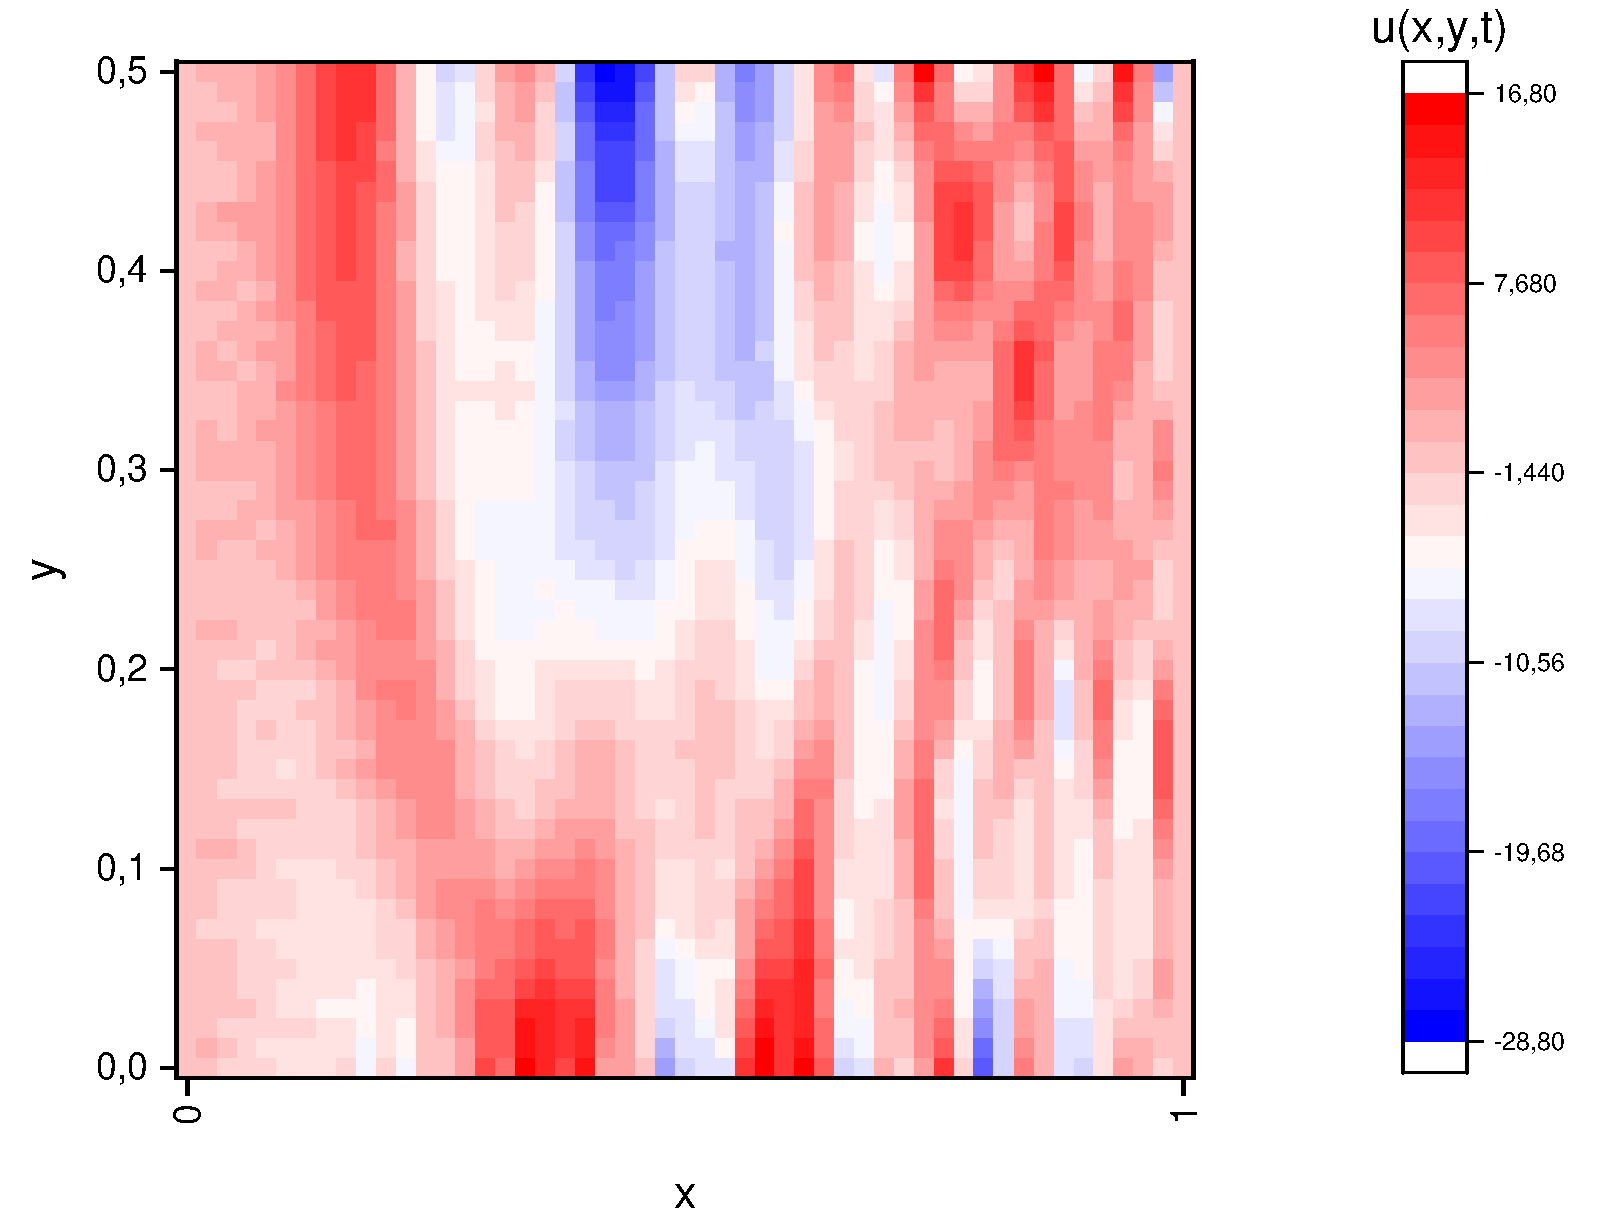
\includegraphics[width=\textwidth]{graphs/graphs_l/v2/wave_t-8_v2.pdf} \begin{center}	b)	\end{center}
		\end{minipage}
		\begin{minipage}[h]{0.23\linewidth}
			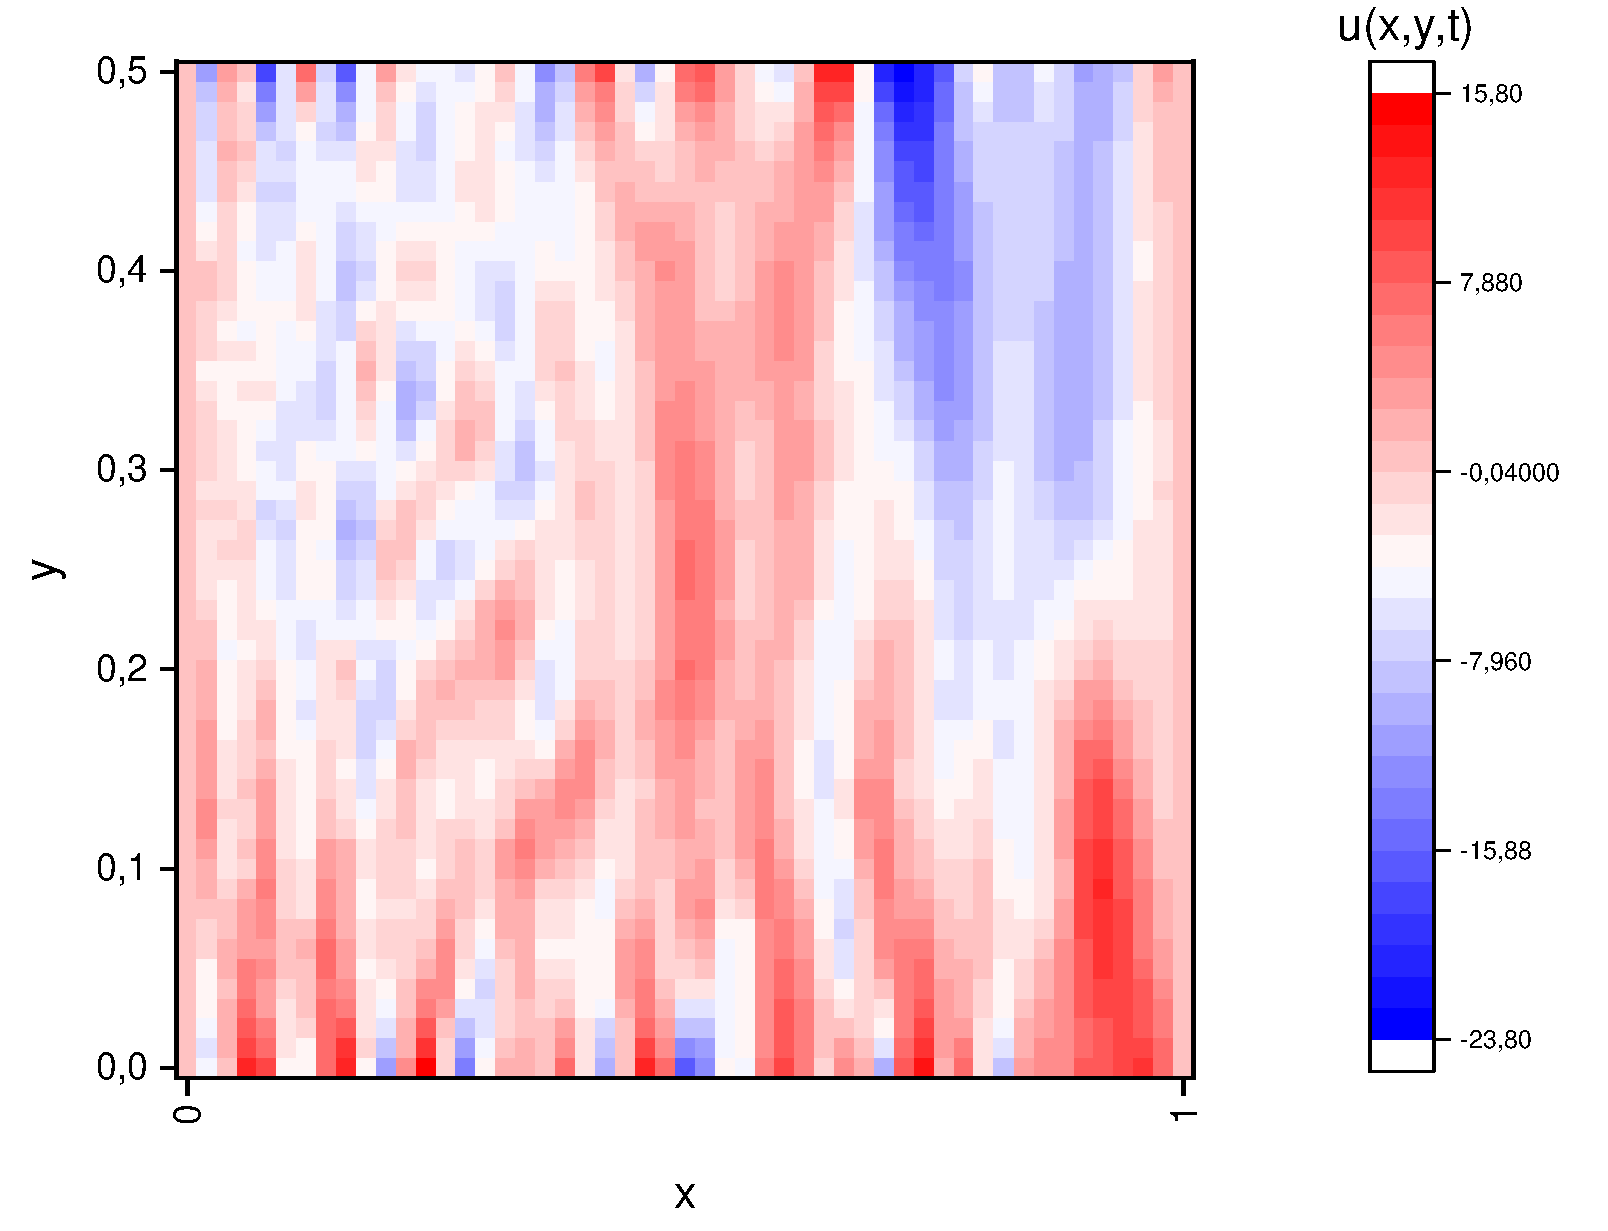
\includegraphics[width=\textwidth]{graphs/graphs_l/v2/wave_t-16_v2.pdf} \begin{center}	c)	\end{center}
		\end{minipage}
		\begin{minipage}[h]{0.23\linewidth}
			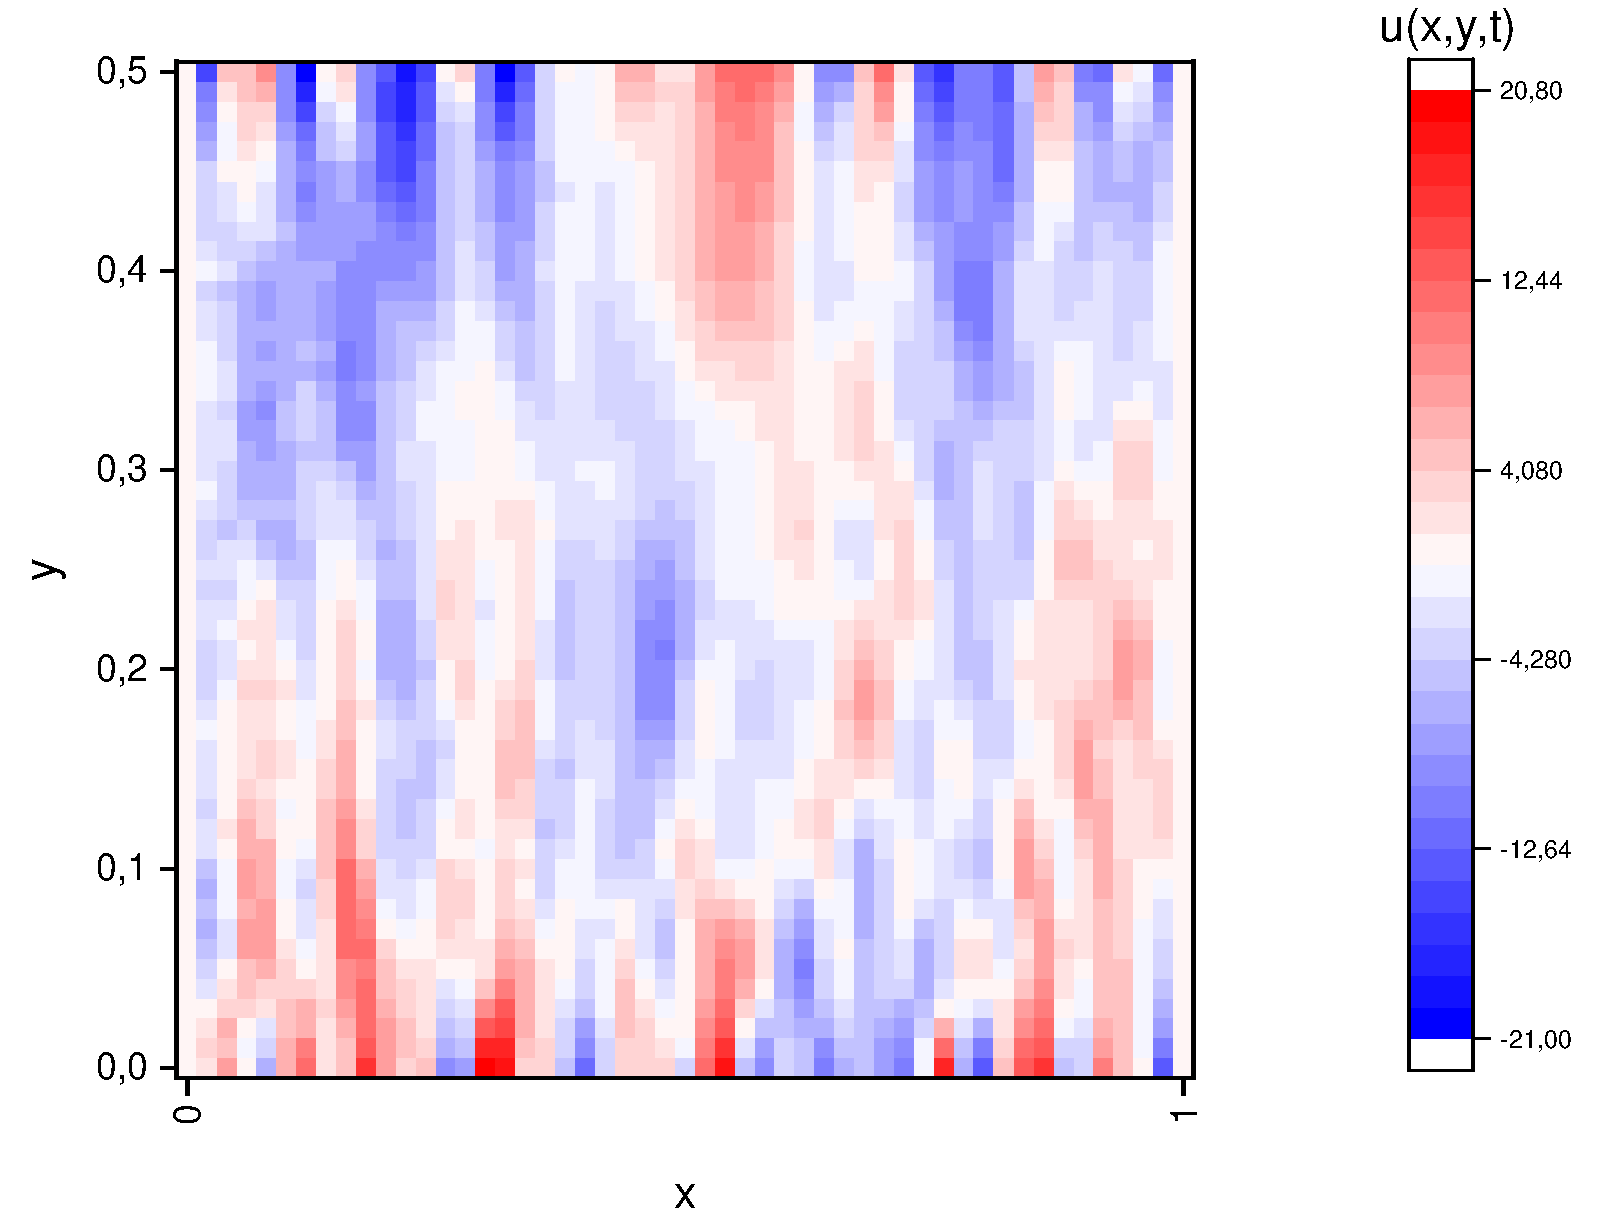
\includegraphics[width=\textwidth]{graphs/graphs_l/v2/wave_t-24_v2.pdf} \begin{center}	d)	\end{center}
		\end{minipage}
	\end{center}
	\caption{Решение для моментов времени (a)$\ t = 0.0$, (b) $\ t = 1.6$, (c)$\ t = 3.2$, (d)$\ t = 4.8$}
\end{figure}

Варианты графиков v2 srez
\begin{figure}[h!]
	\begin{center}
		\begin{minipage}[h]{0.24\linewidth}
			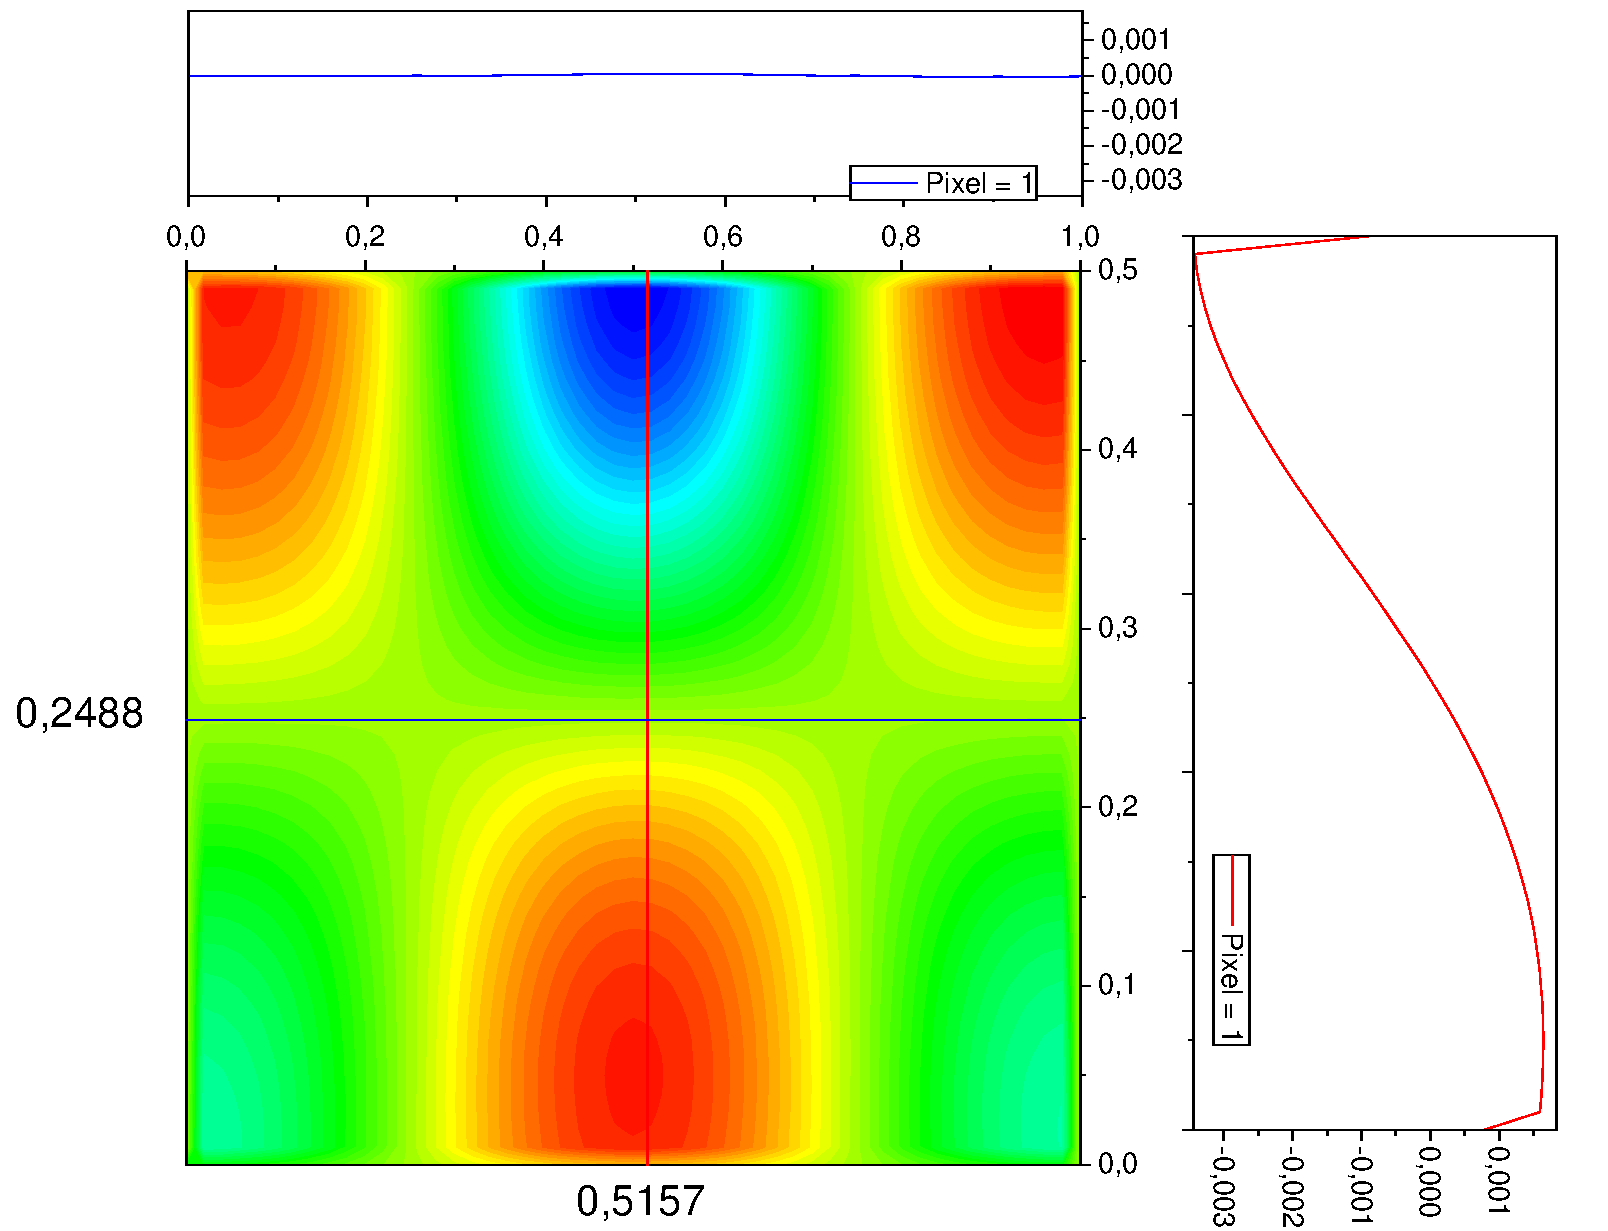
\includegraphics[width=\textwidth]{graphs/graphs_l/v2/wave_t-0_v2_srez} \begin{center}	a)	\end{center}
		\end{minipage}
		\begin{minipage}[h]{0.24\linewidth}
			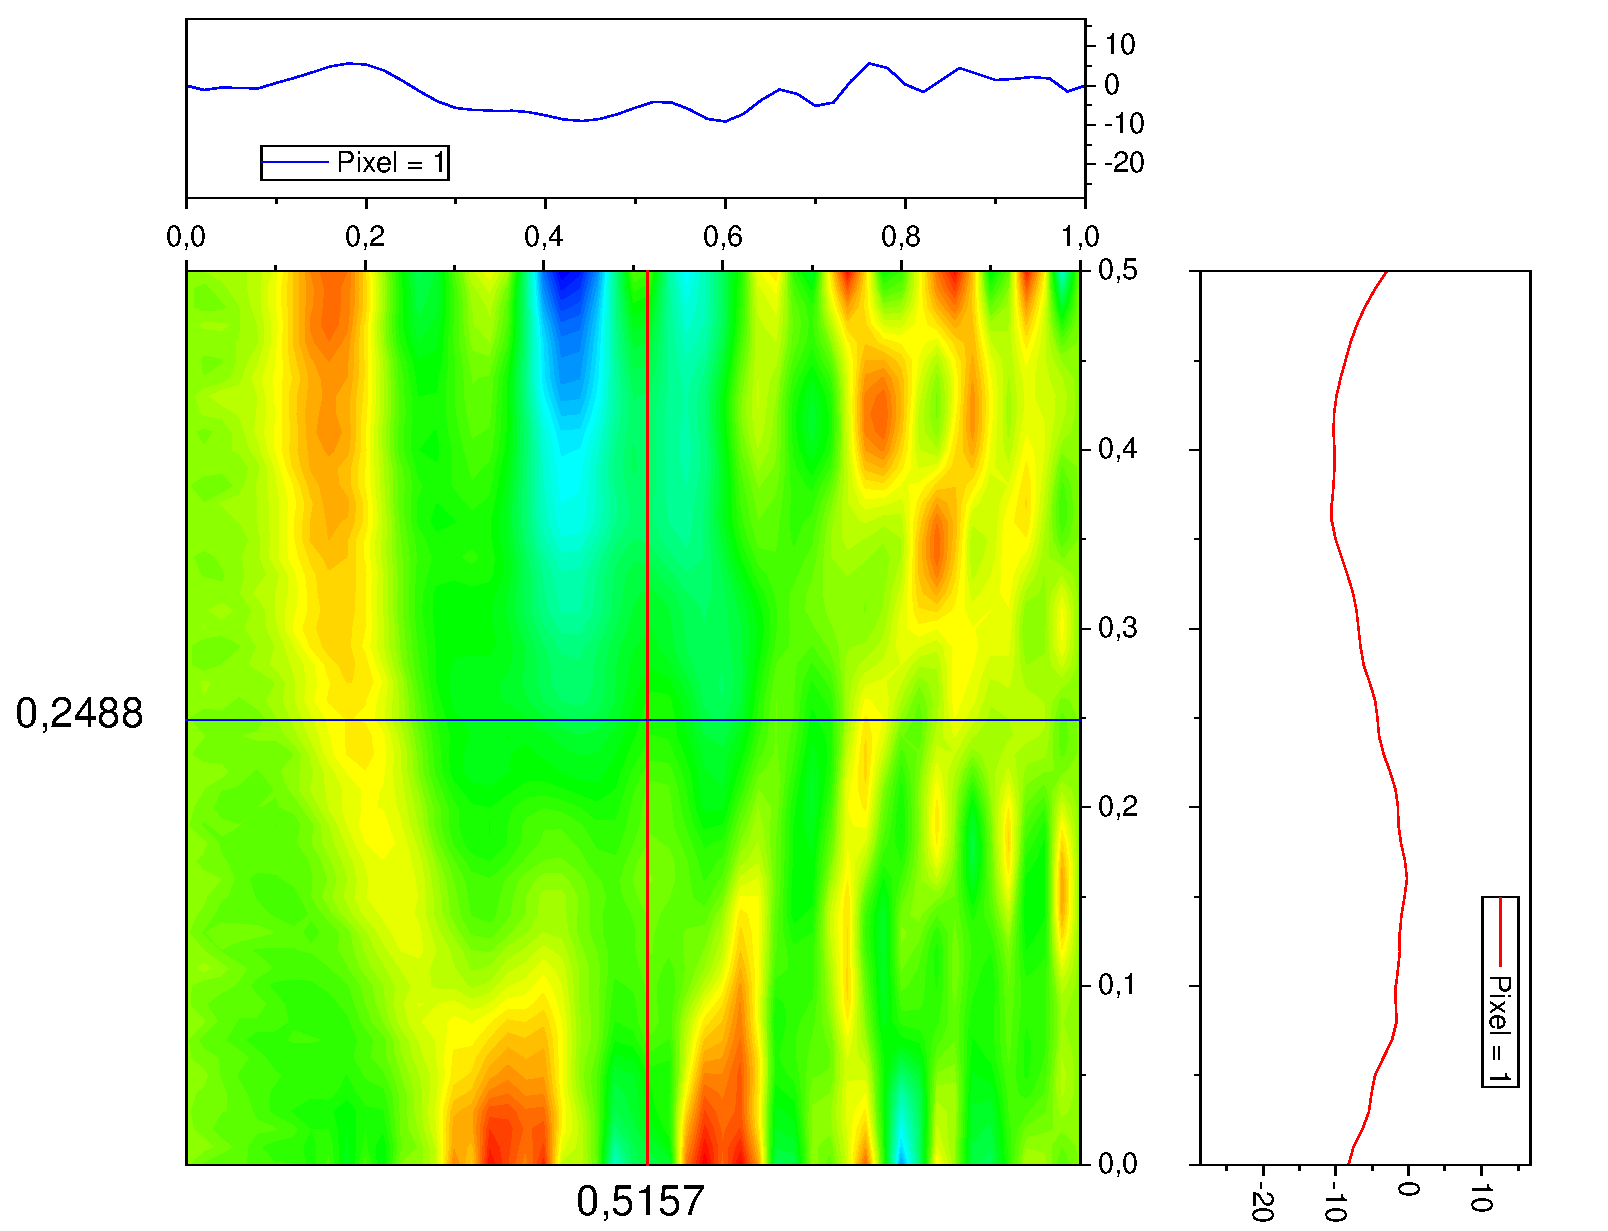
\includegraphics[width=\textwidth]{graphs/graphs_l/v2/wave_t-8_v2_srez} \begin{center}	b)	\end{center}
		\end{minipage}
		\begin{minipage}[h]{0.24\linewidth}
			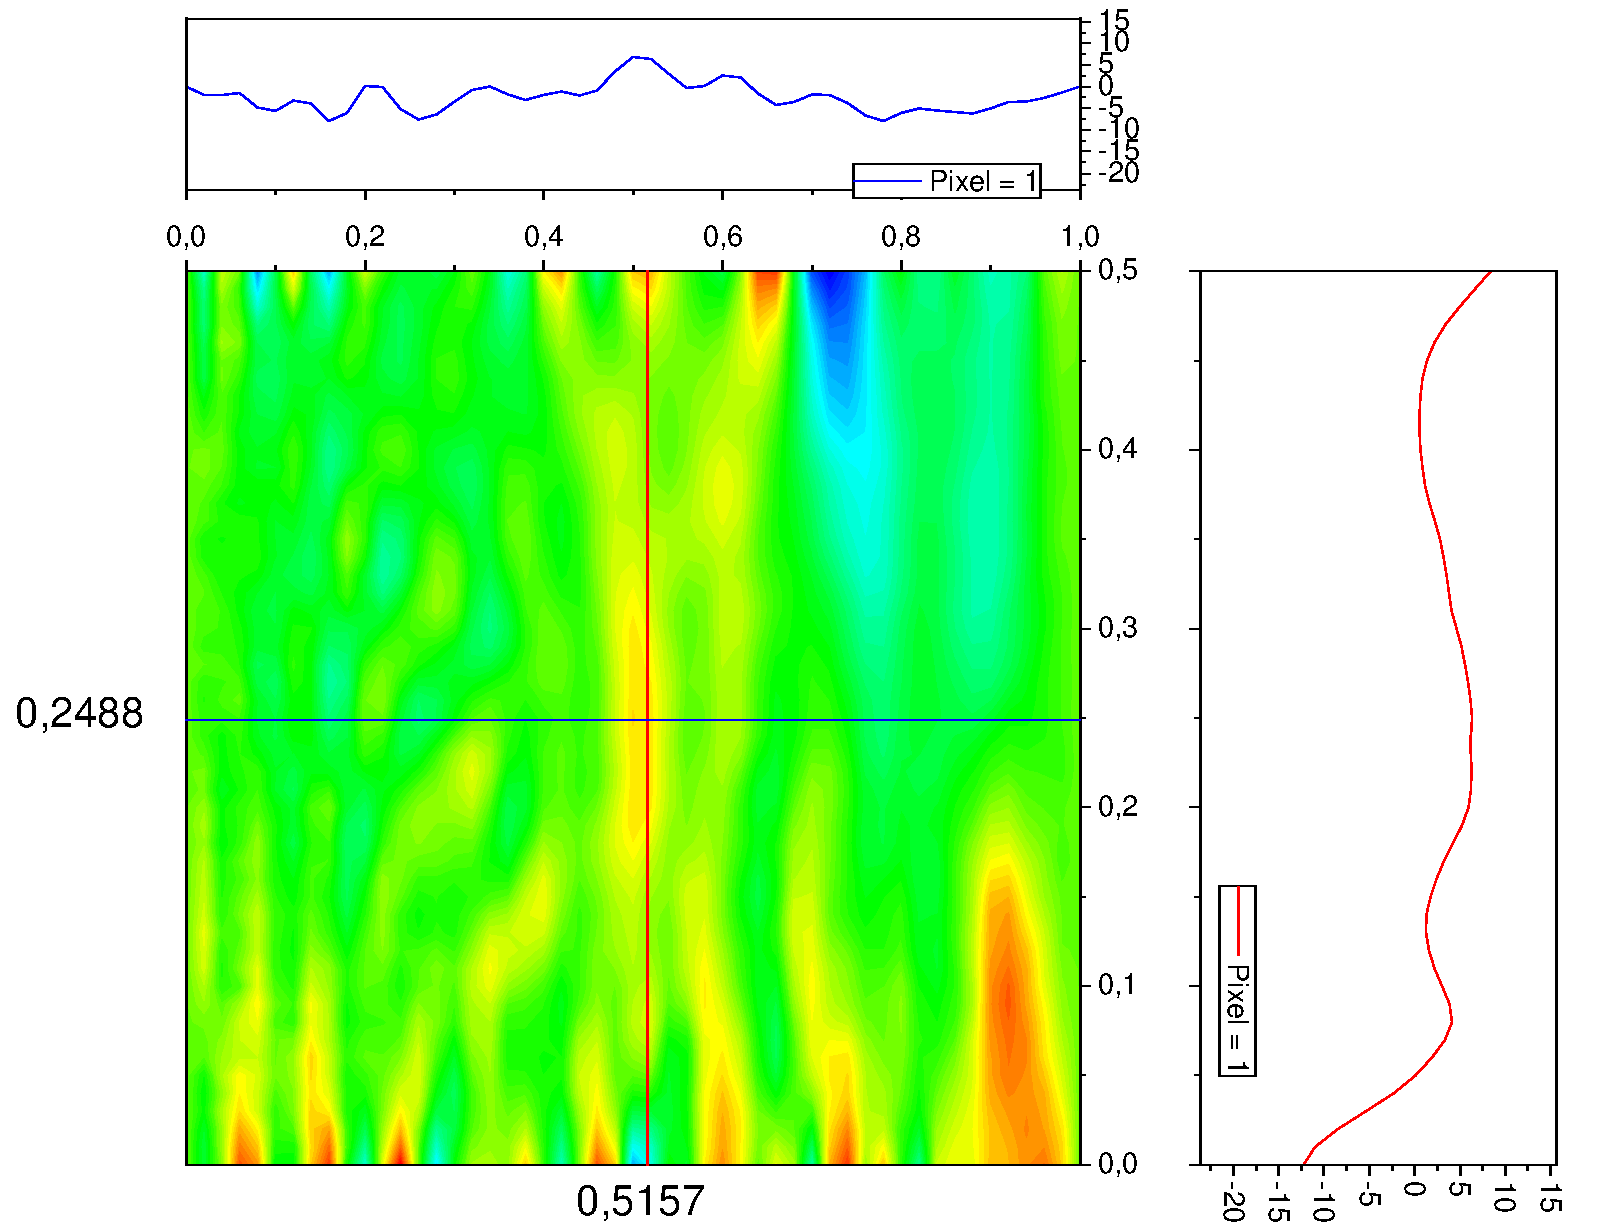
\includegraphics[width=\textwidth]{graphs/graphs_l/v2/wave_t-16_v2_srez} \begin{center}	c)	\end{center}
		\end{minipage}
		\begin{minipage}[h]{0.24\linewidth}
			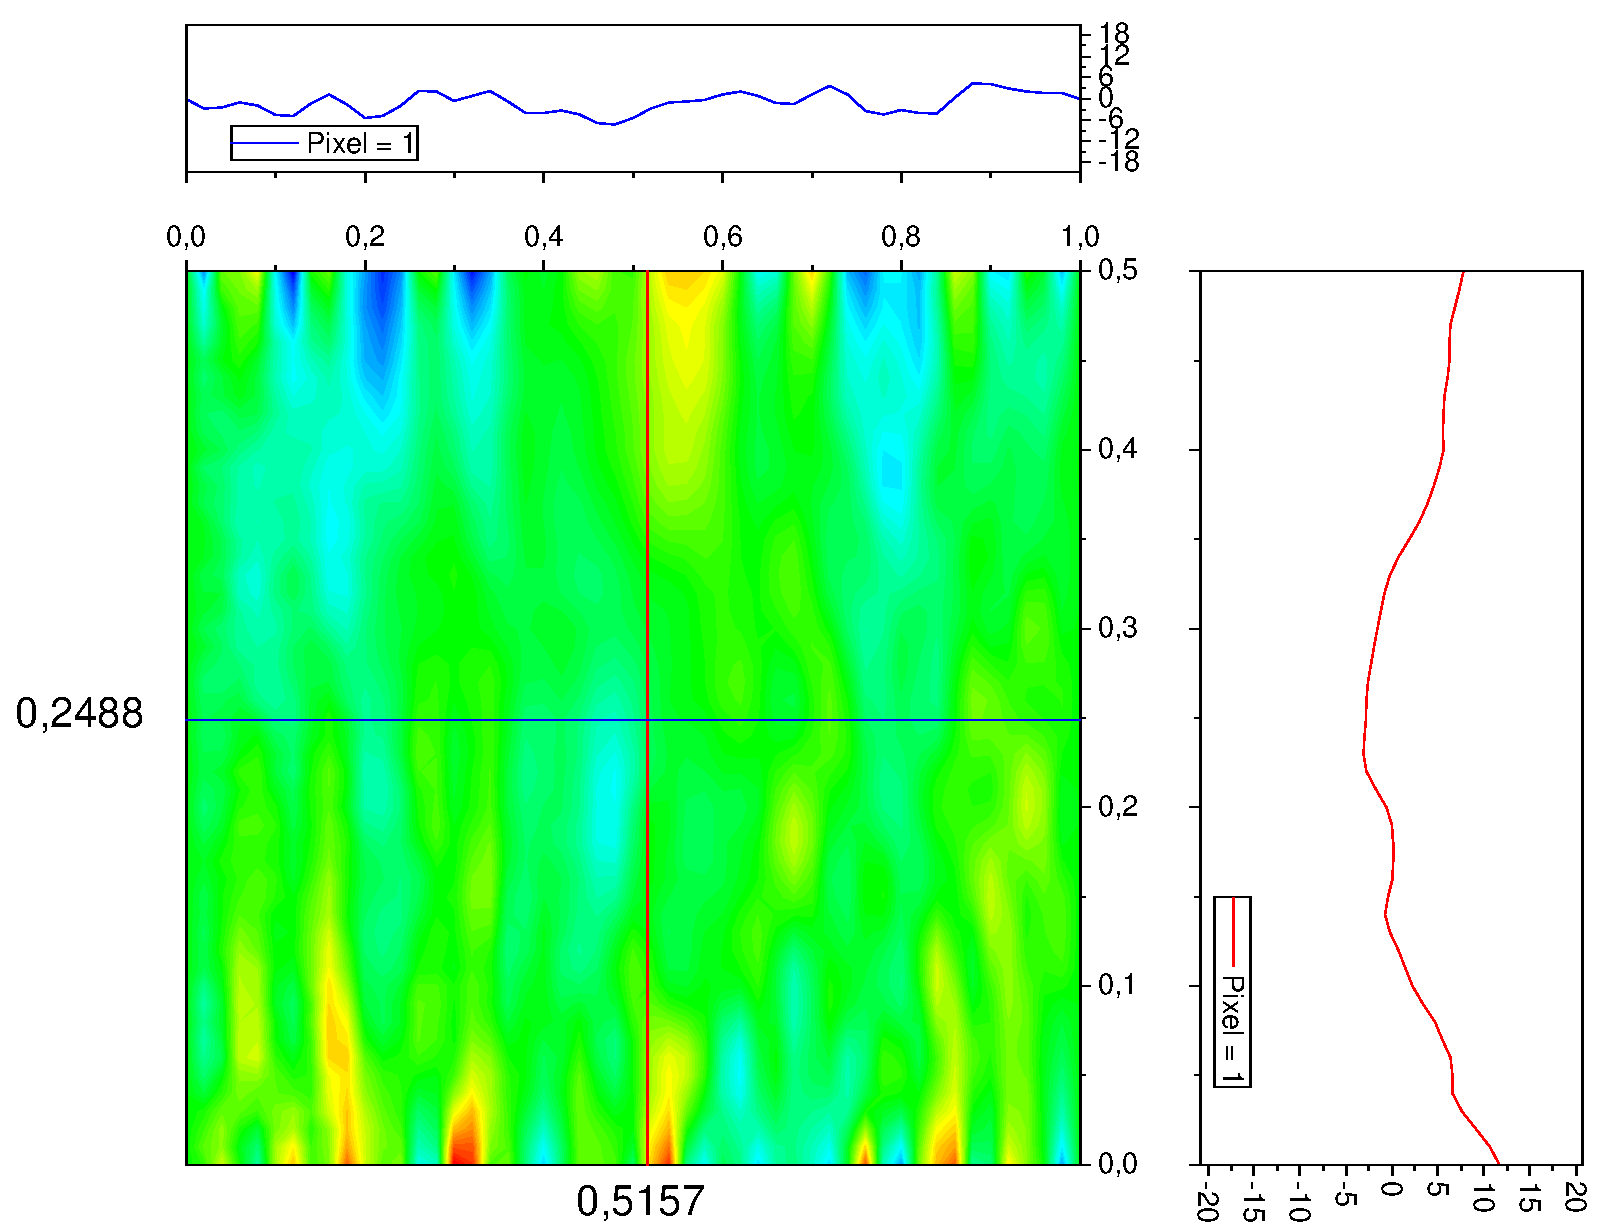
\includegraphics[width=\textwidth]{graphs/graphs_l/v2/wave_t-24_v2_srez} \begin{center}	d)	\end{center}
		\end{minipage}
	\end{center}
	\caption{Срезы решения для моментов времени (a)$\ t = 0.0$, (b) $\ t = 1.6$, (c)$\ t = 3.2$, (d)$\ t = 4.8$}
\end{figure}


%>>>>>>>>>>>>>>>>>>>>>>>>>>>>>>>>>>>>>>>>>>>>>>>>>>>>>>>>>>>>>>>>>>>>>>>>>>>>>>>>>>>>>>>>>>>>>>>>>>>>>>>
\newpage
\section*{Заключение}
\addcontentsline{toc}{section}{Заключение}
В данной работе были рассмотрены:
 \begin{enumerate}
 	\item Тестовая краевая задача. Построены зависимости $u(x) = u(\textbf{r} , t)$, построены срезы.
 	\item Индивидуальная задача. Получено решение индивидуального задания с краевой задачей для волнового уравнения$(2 - 15)$.
 	Построены зависимости решения \qquad $u = u(r, t)$ от координат $r$ для нескольких значений временной зависимости $t$.
 \end{enumerate}
Для решения граничной задачи был реализован метод прямых. Задача Коши решается многошаговым методом Адамса-Мултона со стартовым методом Лобатто $IIIC$ второго порядка точности.\\

%>>>>>>>>>>>>>>>>>>>>>>>>>>>>>>>>>>>>>>>>>>>>>>>>>>>>>>>>>>>>>>>>>>>>>>>>>>>>>>>>>>>>>>>>>>>>>>>>>>>>>>>

\newpage
\addcontentsline{toc}{section}{Список литературы}
\begin{thebibliography}{99}

\bibitem{Kalitkin_2013_1}
Калиткин Н.Н., Альшина Е.А., Корякин П.В. 
Численные методы. Книга 1. Численный анализ. --- М.: Академия, 2013. 

\bibitem{Kalitkin_2013_2}
Калиткин Н.Н., Корякин П.В. 
Численные методы. Книга 2. Методы математической физики. --- М.: Академия, 2013. 

\bibitem{Kalitkin_BJK_2003}
Бахвалов Н.С., Жидков Н.П., Кобельков Г.М. 
Численные методы. --- М.: Бином, 2003, 2012.

\bibitem{HNW_I}
Хайрер Э., Нёрсетт С., Ваннер Г. 
Решение обыкновенных дифференциальных уравнений. 
Нежесткие задачи. --- М.: Мир, 1990.

\bibitem{HNW_II}
Хайрер Э., Ваннер Г. 
Решение обыкновенных дифференциальных уравнений. 
Жесткие и дифференциально-алгебраические задачи. --- М.: Мир, 1999.

\bibitem{Butcher_2016}
Butcher J.C. Numerical Methods for Ordinary Differential Equations. --- 
John Wiley \& Sons, 2016.

\end{thebibliography}
\end{document}